
\chapter[Case studies]{Case studies}
\graphicspath{ {images/casestudies} }

This chapter presents an actual case use scenario of SYN applied to open-source software systems. 
We use SYN to analyze the evolution of JetUML, the test project on which we relied during the development phase of the platform, ArgoUML, Elasticsearch, and Linux. 
The characteristics of these systems are described in \autoref{tab:casestudies}

\begin{table}[ht]
    \centering
    \begin{tabular}{lcrr} 
        \hline
        {\bf Name} & {\bf First Analyzed Commit} & {\bf Last Analyzed Commit} & {\bf \# of commits}\\ 
        \hline
        JetUML & Wed Jan 07 2015 &  Thu May 12 2022  &  2152  
    \end{tabular}
    \caption{List of analyzed projects}
    \label{tab:casestudies}
\end{table}

\bigbreak
There are many possible combinations to create a view specification; we explored them on all the projects. 
Each visualization has its purpose. For example, we can create a visualization to see the evolution of only Java files, or we can create a visualization to see how the system evolved every day. 
However, not all the combinations might have sense. For example, if we chose a timestamp grouping strategy, the time window must be chosen conscientiously. 
A comprehensive time window might hide some exciting aspects of the analysis. In contrast, a short time window could cause a massive number of AnimationFrames, undermining the understandability of the view. 
\bigbreak
A constant factor of all our visualization is the choice not to show deleted entities, the adoption of a LinearBucketValueStrategy for the mapper with a maximum height of 20, and finally, to display files that do not have the selected metric on the visualization. 
These properties are set as follow:
\begin{itemize}
    \item \texttt{showUnmappedEntities}: true.
    \item \texttt{mapperStrategy}: LinearBucketValueStrategy.
    \item \texttt{mapperStrategyOptions}: max height of 20.
    \item \texttt{showDeletedEntities}: false.
\end{itemize}
This choice is because, during the development process, we have seen that the LinearBucketValueStrategy works better than other strategies. Of course, it needs a maximum height because otherwise, the gap between entities is too broad. Therefore set this value to 20. Moreover, we believe that hiding the deleted entities is the most intuitive thing for the user. On the other hand, hiding unmapped entities might be misleading in some visualization. This is why we preferred to keep them. 

\subsection{JetUML}
This section analyzes JetUML, an open-source desktop application to work with UML diagrams.
The main development branch is composed of 2152 commits of 24 contributors. 

\subsubsection{View 1}
\begin{figure}[t!]
    \begin{subfigure}{0.42\textwidth}
        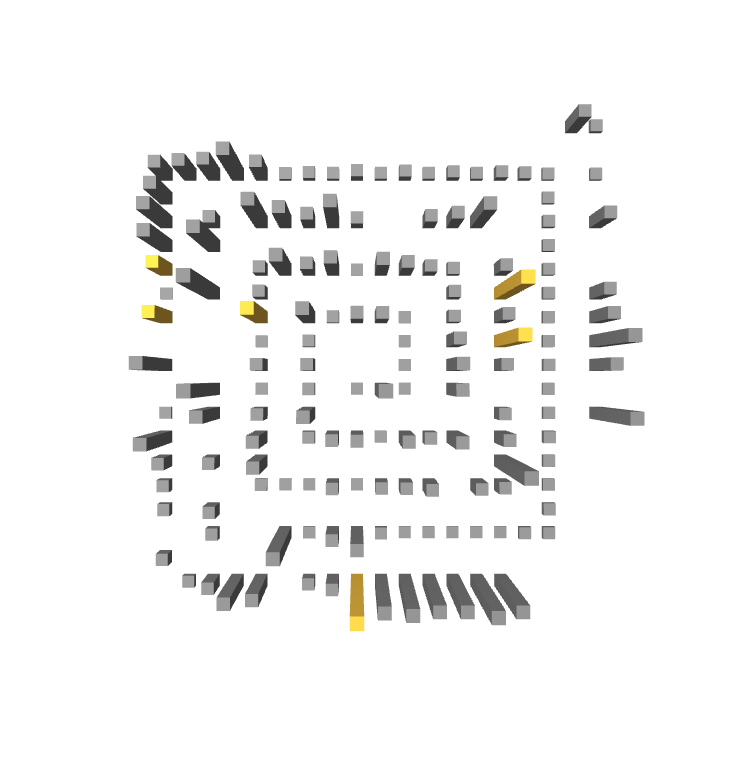
\includegraphics[width=\linewidth]{JetUML_V0E0.png}
        \caption{Commit that involved few entities} \label{fig:JetUML_V0E0}
    \end{subfigure}
    \hspace*{\fill}
    \begin{subfigure}{0.42\textwidth}
        
\includegraphics[width=\linewidth]{JetUML_V0E1.png}
        \caption{Commit that involved numerous entities} \label{fig:JetUML_V0E1}
    \end{subfigure}
    \caption{Comparison of comits with a low and an hight activity} 
    \label{fig:JetUML_V0E0}
\end{figure}

\textbf{Goal of this visualization} Visualize the entire repository commit by commit to see how the repository evolved and understand commits with high activity. 
To highlight them, we use a commit aging strategy, where the next age is reached after one commit with a maximum age of two.
Consequently, all the files not included in the depicted commit are painted with the base color (gray by default). 

Figure \ref{fig:JetUML_V0E0} shows the graphical difference between commits that modified a few entities and commits that changed numerous entities. 
To identify highly active commits, we focused our attention on commits that have involved a large number of entities. 

The view specification of this visualization is the following
\begin{itemize}
    \item \texttt{versionGroupingStrategy}: commit.
    \item \texttt{versionGroupingChunkSize}: 1. 
    \item \texttt{colorPalette}: default.
    \item \texttt{agingGroupingStrategy}: commit.
    \item \texttt{agingStepSize}: 1.
    \item \texttt{agingSteps}: 2 steps. 
    \item \texttt{mapperMetricName}: SIZE. 
    \item \texttt{fileTypeShape}: all boxes.
    \item \texttt{fileTypeOpacity}: all 1. 
\end{itemize}

\textbf{Results}

\begin{figure}[h!]
    \begin{subfigure}{0.42\textwidth}
        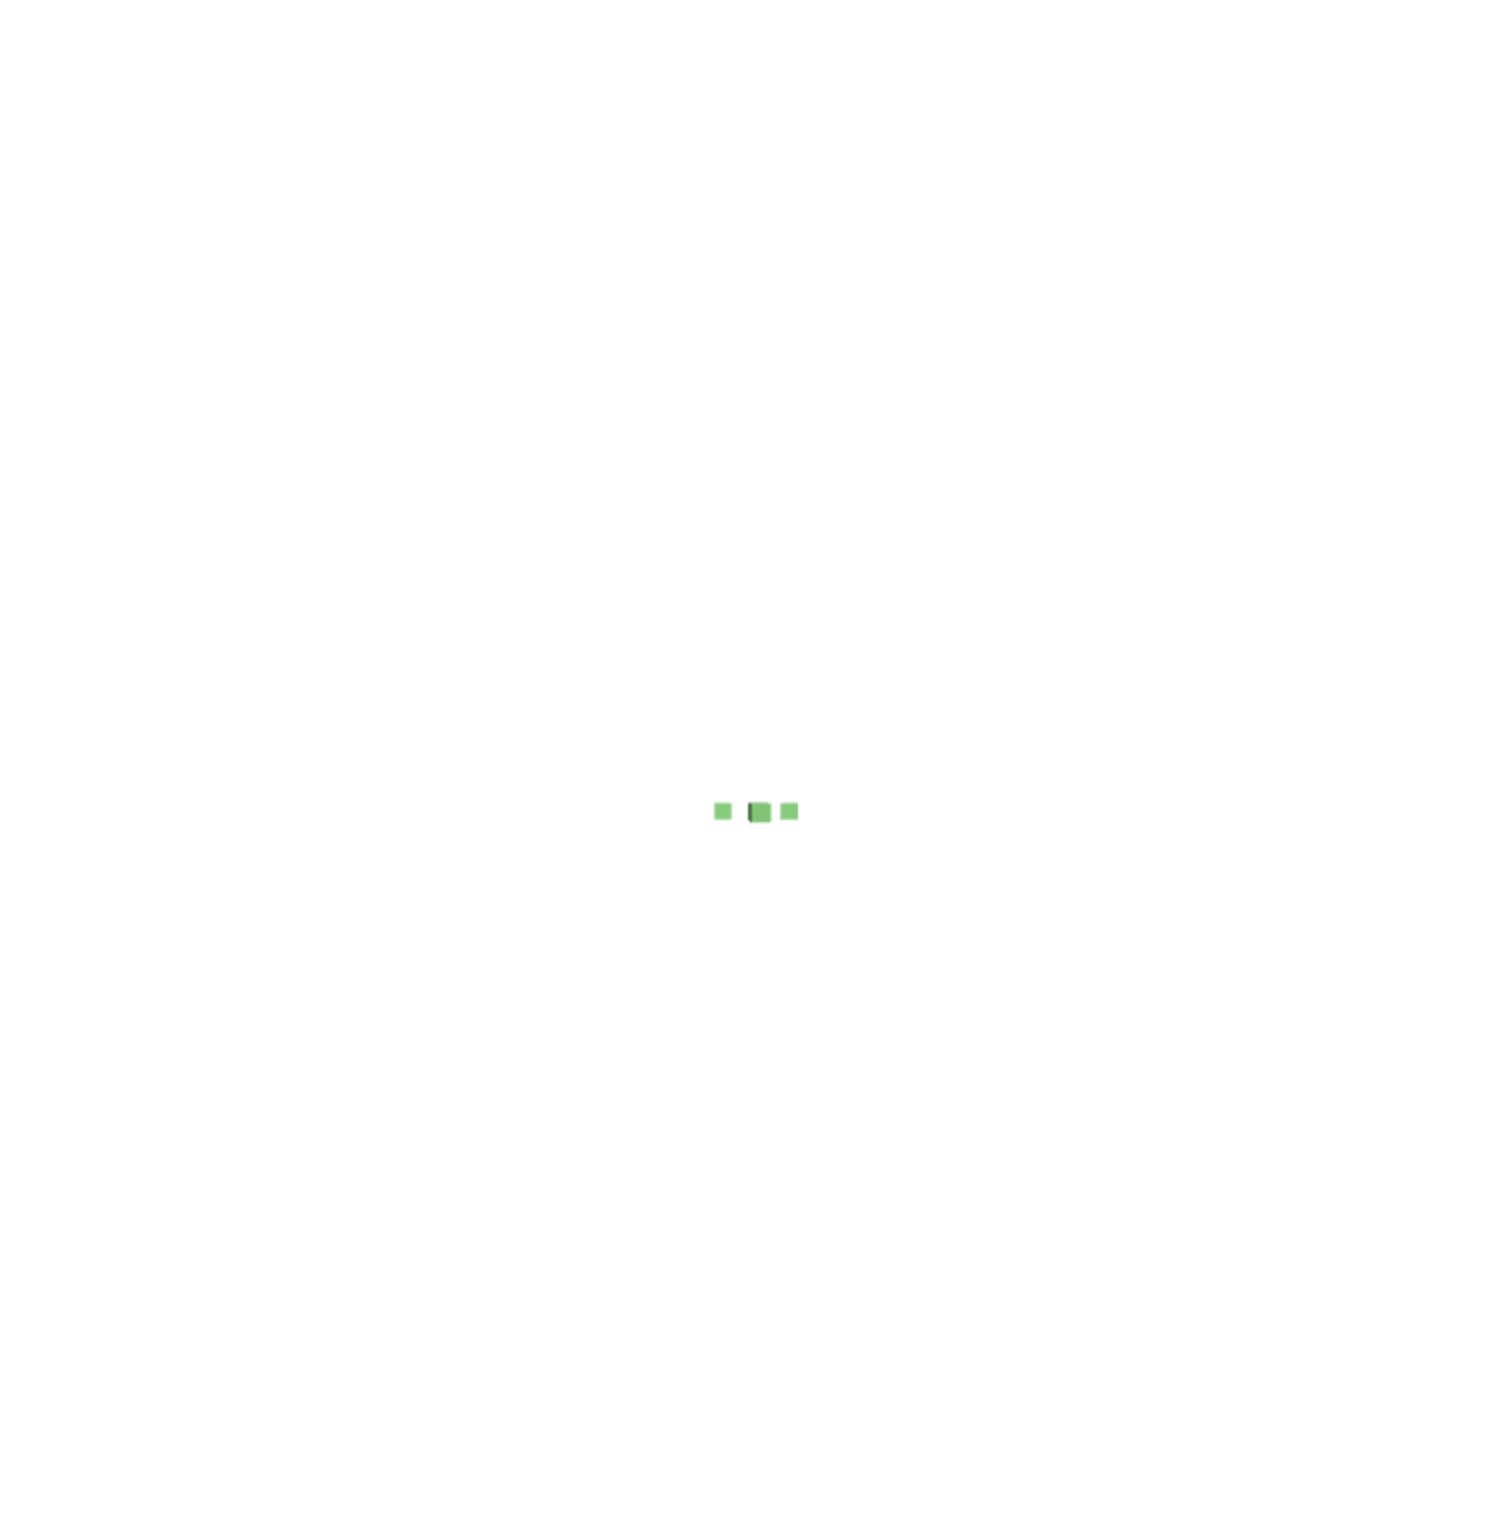
\includegraphics[width=\linewidth]{JetUML_V0S1.png}
        \caption{First commit seen from a top angle } 
        \label{fig:JetUML_V0S1_0}
    \end{subfigure}
    \hspace*{\fill}
    \begin{subfigure}{0.42\textwidth}
        
\includegraphics[width=\linewidth]{JetUML_V0S1_1.png}
        \caption{First commit seen from a mid angle} 
        \label{fig:JetUML_V0S1_1}
    \end{subfigure}
    \caption{First commit of JetUML made on Wed, 07 Jan 2015, 18:59. Three entities have been added; they are depicted with the green color. The entity in the middle represents the license file, taller because its size is bigger than other files.} 
    \label{fig:JetUML_V0S1}
\end{figure}

Here we present some results that we found looking at the graphical evolution of JetUML. 
To keep this section short, we report only a subset of the most active commits below. 
\bigbreak
The repository's history starts on January 7, 2015, when Martin Robillard made the first commit. 
This commit added three files: README, a license, and a gitingore. 
Figure \ref{fig:JetUML_V0S1} represents it with three entities. They all have the same shape because we did not adopt different shapes in the specification, but the height is different. The license file is taller than other entities because of its bigger size. 
\bigbreak
Fifteen minutes later, he pushed the initial codebase of a project named Violet, composed of 83 files and an updated version of the gitignore file. This commit is represented in figure \ref{fig:JetUML_V0S2}, where 83 green entities represent added files, one yellow entity represents the updated gitignore files, and two gray entities, the README and the license files added before, that were not touched.
\bigbreak
Forty minutes later, he made the first big refactor of the system, whose goal was to move the position of some fields in each class. This refactoring involved 49 files, and as we can see from figure \ref{fig:JetUML_V0S3} they are marked in yellow. 
\bigbreak
Three days later, after a series of delicate development tasks had been continuously made, he moved some classes from the Violet folder to a new one named Violetta. As we can notice from figure \ref{fig:JetUML_V0S4} moved classes are represented with light blue. 
\bigbreak
Twenty-six commits later, on January 22, 2015, they moved classes from Violet and Violetta under the JetUML package. This commit, represented in figure \ref{fig:JetUML_V0S5}, was the first when JetUML was officially used; it denotes its birth. 
\bigbreak
After this first implementation, the system gradually grew, doubling its size in less than two years. 
During this time interval, they have been made only small commits to solve open issues. There were some exceptions, displayed in figure \ref{fig:JetUML_V0S6} and \ref{fig:JetUML_V0S7} where many files were modified because they had to update classes copyright lines. 
\bigbreak
In November 2017, they removed "stg" from the path of all the Java classes part of the system. This commit is depicted in figure \ref{fig:JetUML_V0S8}, where we can observe 162 light blue entities. They represent classes moved from the "../ca/mcgill/cs/stg/jetuml/..." path to the 
"../ca/mcgill/cs/jetuml/..." path. Moreover, this commit also had 15 modified fields, and one added. 
\bigbreak
One last huge refactor was done in July 2020, two years later, again to change the copyright on every class. It is represented in figure \ref{fig:JetUML_V0S9}. In this figure, we can notice that there are many blank spots in the middle. This means that entities added in the early stages of the project have been removed and are no longer part of the system. At that time, the system had 316 entities, and 241 were affected by this commit. 
\bigbreak
The last version of the system, created on Thu, 12 May 2022, counts 456 entities. 
\bigbreak
\textbf{Conclusion}
We manually inspected 2153 frames depicting the evolution of JetUML.
Thanks to the autoplay feature of SYN-Debugger, it was not an agonizing activity. \\
Occasionally JetUML needed to make huge commits involving most files on their repository. Nonetheless, they were spotted easily, thanks to the adopted visualization settings. 
Most of the commits involved few entities; this means that features were implemented gradually, maybe following an incremental or spiral development approach. 
With this grouping strategy, it was hard to understand the regularity and the speed of the development process. This is normal when we traverse the history by commit rather than traverse it by time. 

\begin{figure}[h!]
    \begin{subfigure}{0.32\textwidth}
        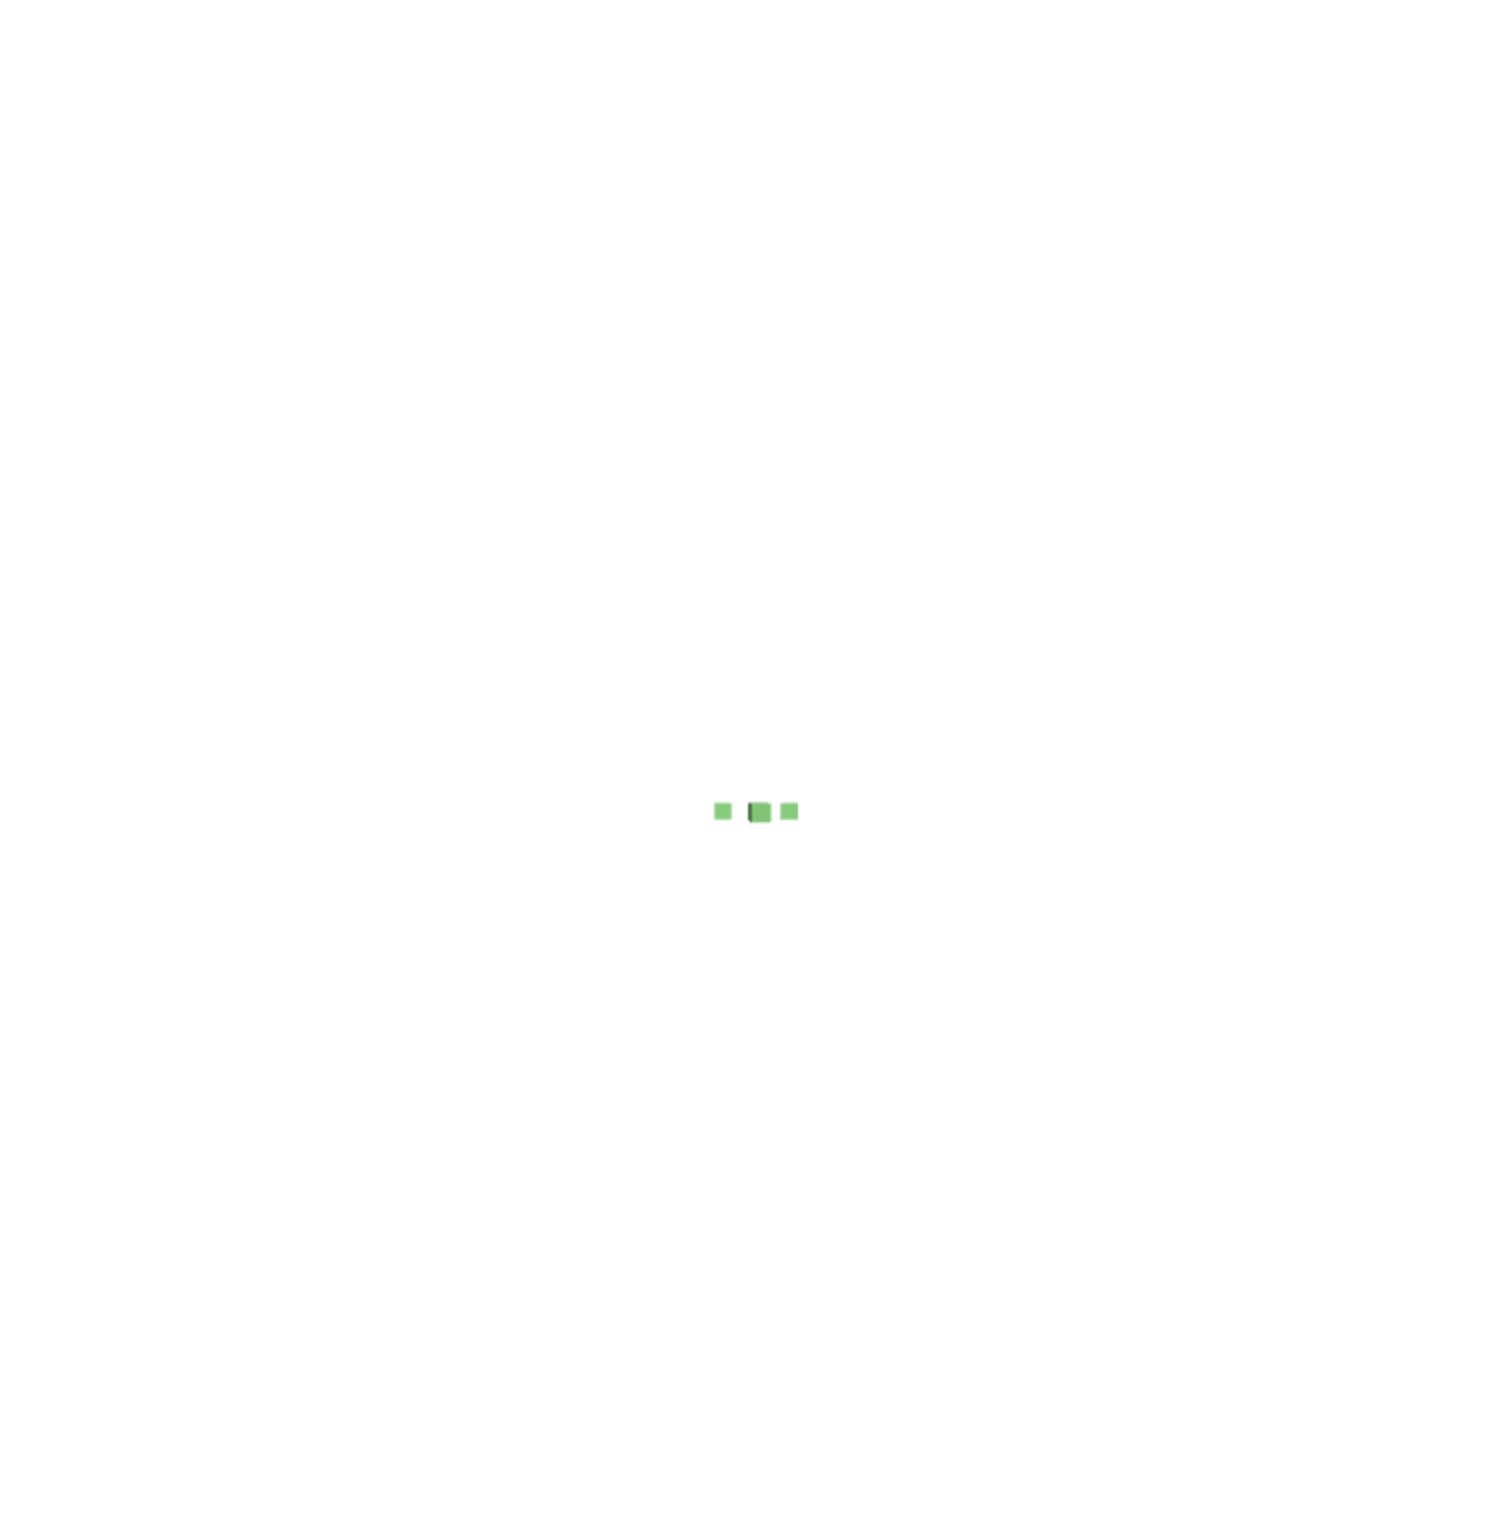
\includegraphics[width=\linewidth]{JetUML_V0S1.png}
        \caption{07 Jan 2015, 18:59 \linebreak Initial commit} 
        \label{fig:JetUML_V0S1_3}
    \end{subfigure}
    \hspace*{\fill}
    \begin{subfigure}{0.32\textwidth}
        
\includegraphics[width=\linewidth]{JetUML_V0S2.png}
        \caption{07 Jan 2015, 19:14 \linebreak  Initial Revision} 
        \label{fig:JetUML_V0S2}
    \end{subfigure}
    \hspace*{\fill}
    \begin{subfigure}{0.32\textwidth}
        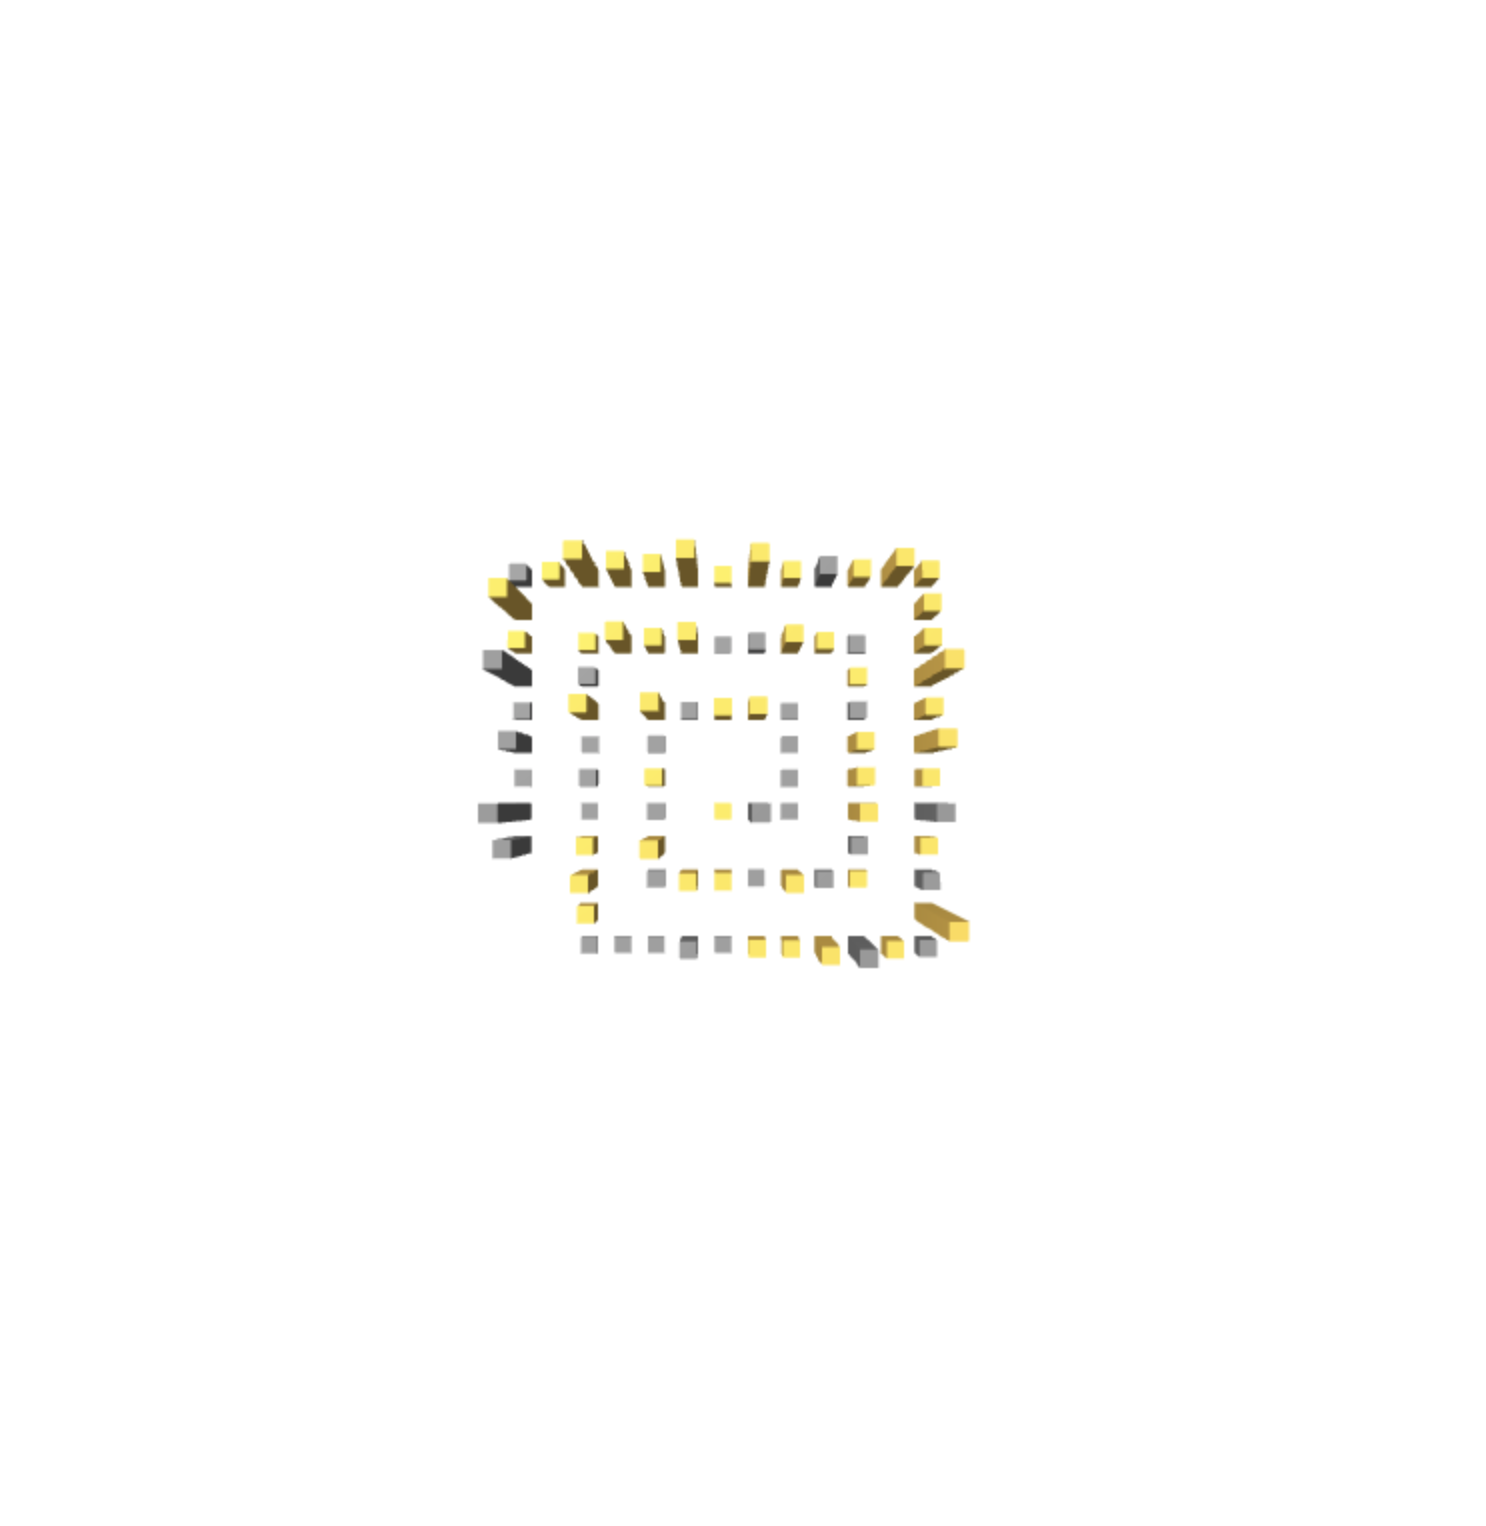
\includegraphics[width=\linewidth]{JetUML_V0S3.png}
        \caption{07 Jan 2015, 19:57 \linebreak  \#1 Move all fields} 
        \label{fig:JetUML_V0S3}
    \end{subfigure}
    \hspace*{\fill}
    \medskip
    \begin{subfigure}{0.32\textwidth}
        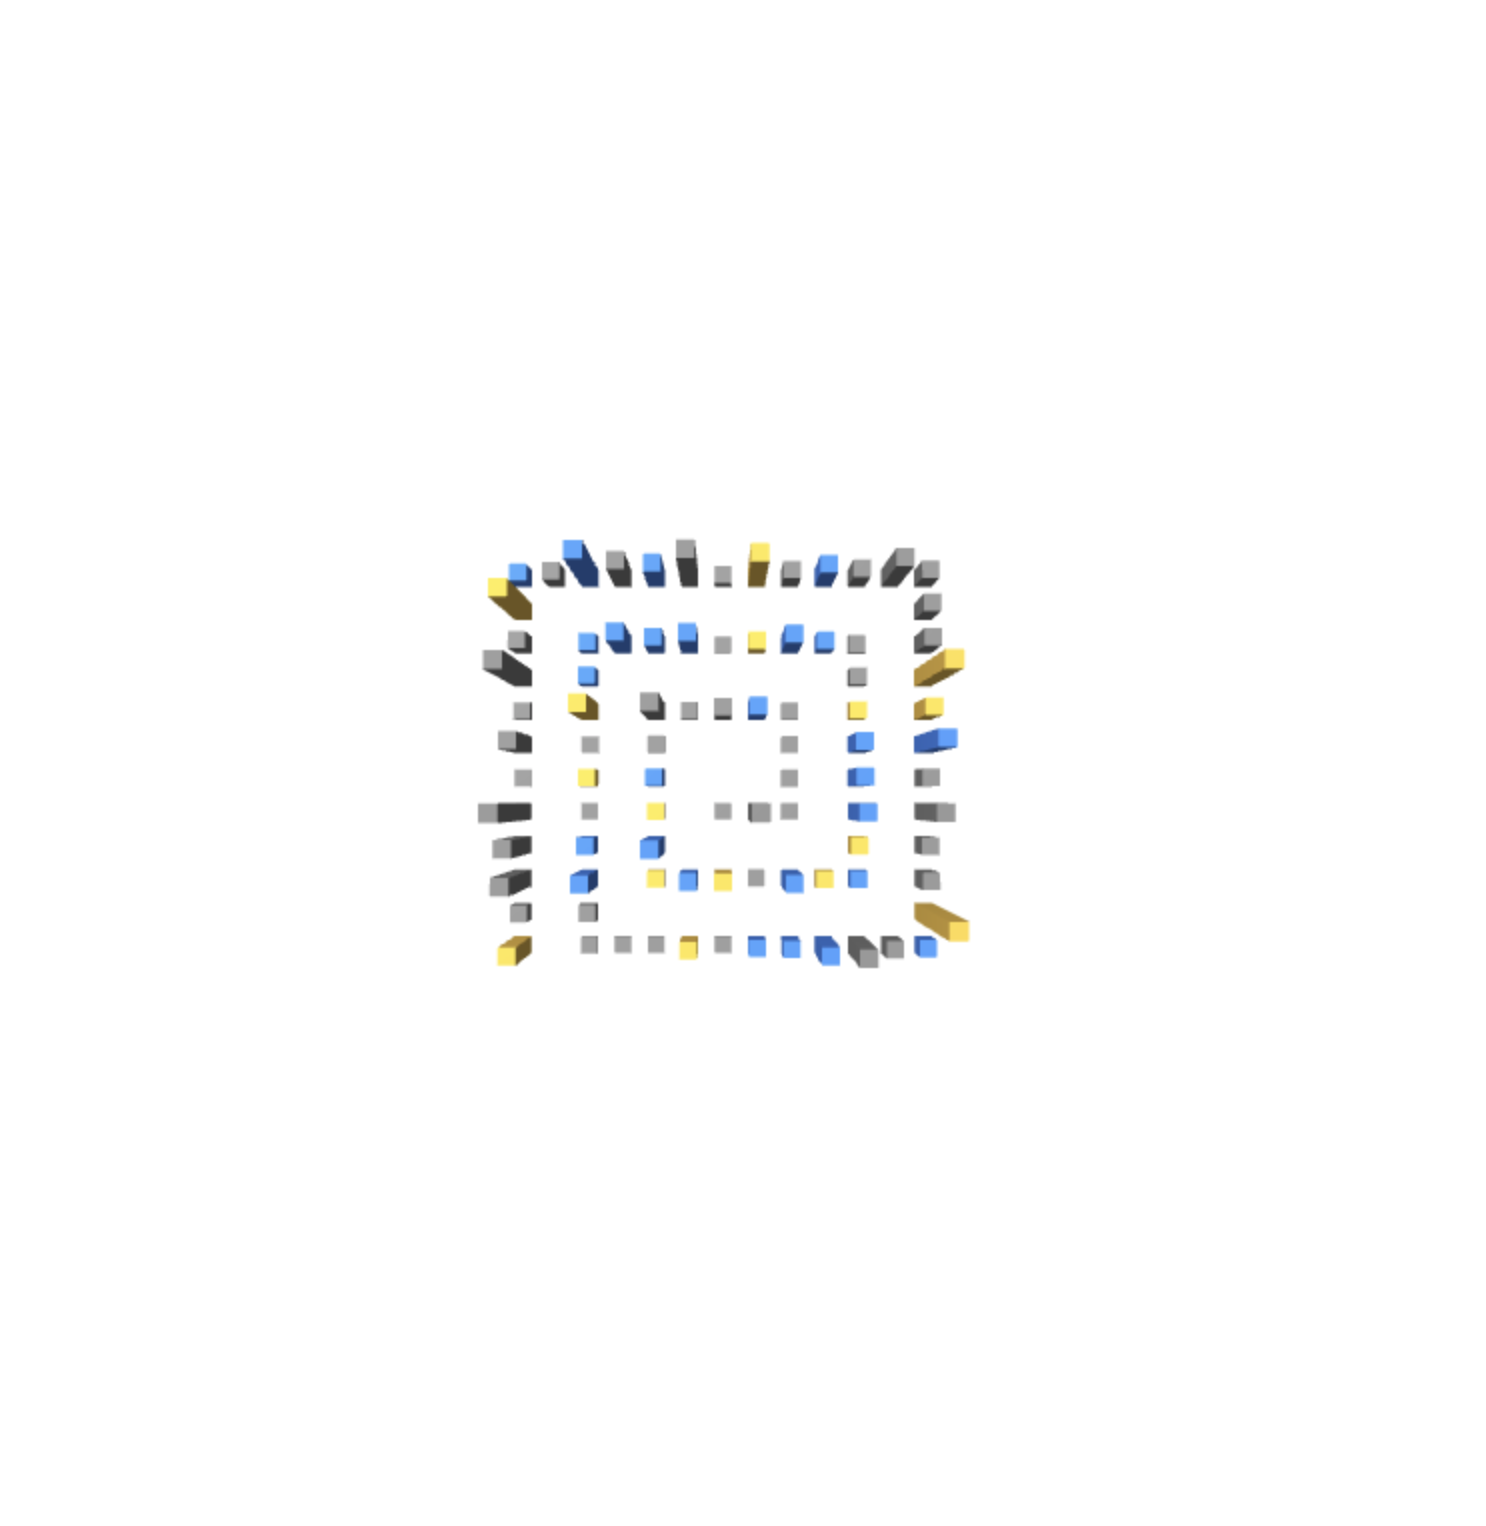
\includegraphics[width=\linewidth]{JetUML_V0S4.png}
        \caption{10 Jan 2015 \linebreak  \#8 Moved to a dedicated ...} 
        \label{fig:JetUML_V0S4}
    \end{subfigure}
    \hspace*{\fill}
    \begin{subfigure}{0.32\textwidth}
        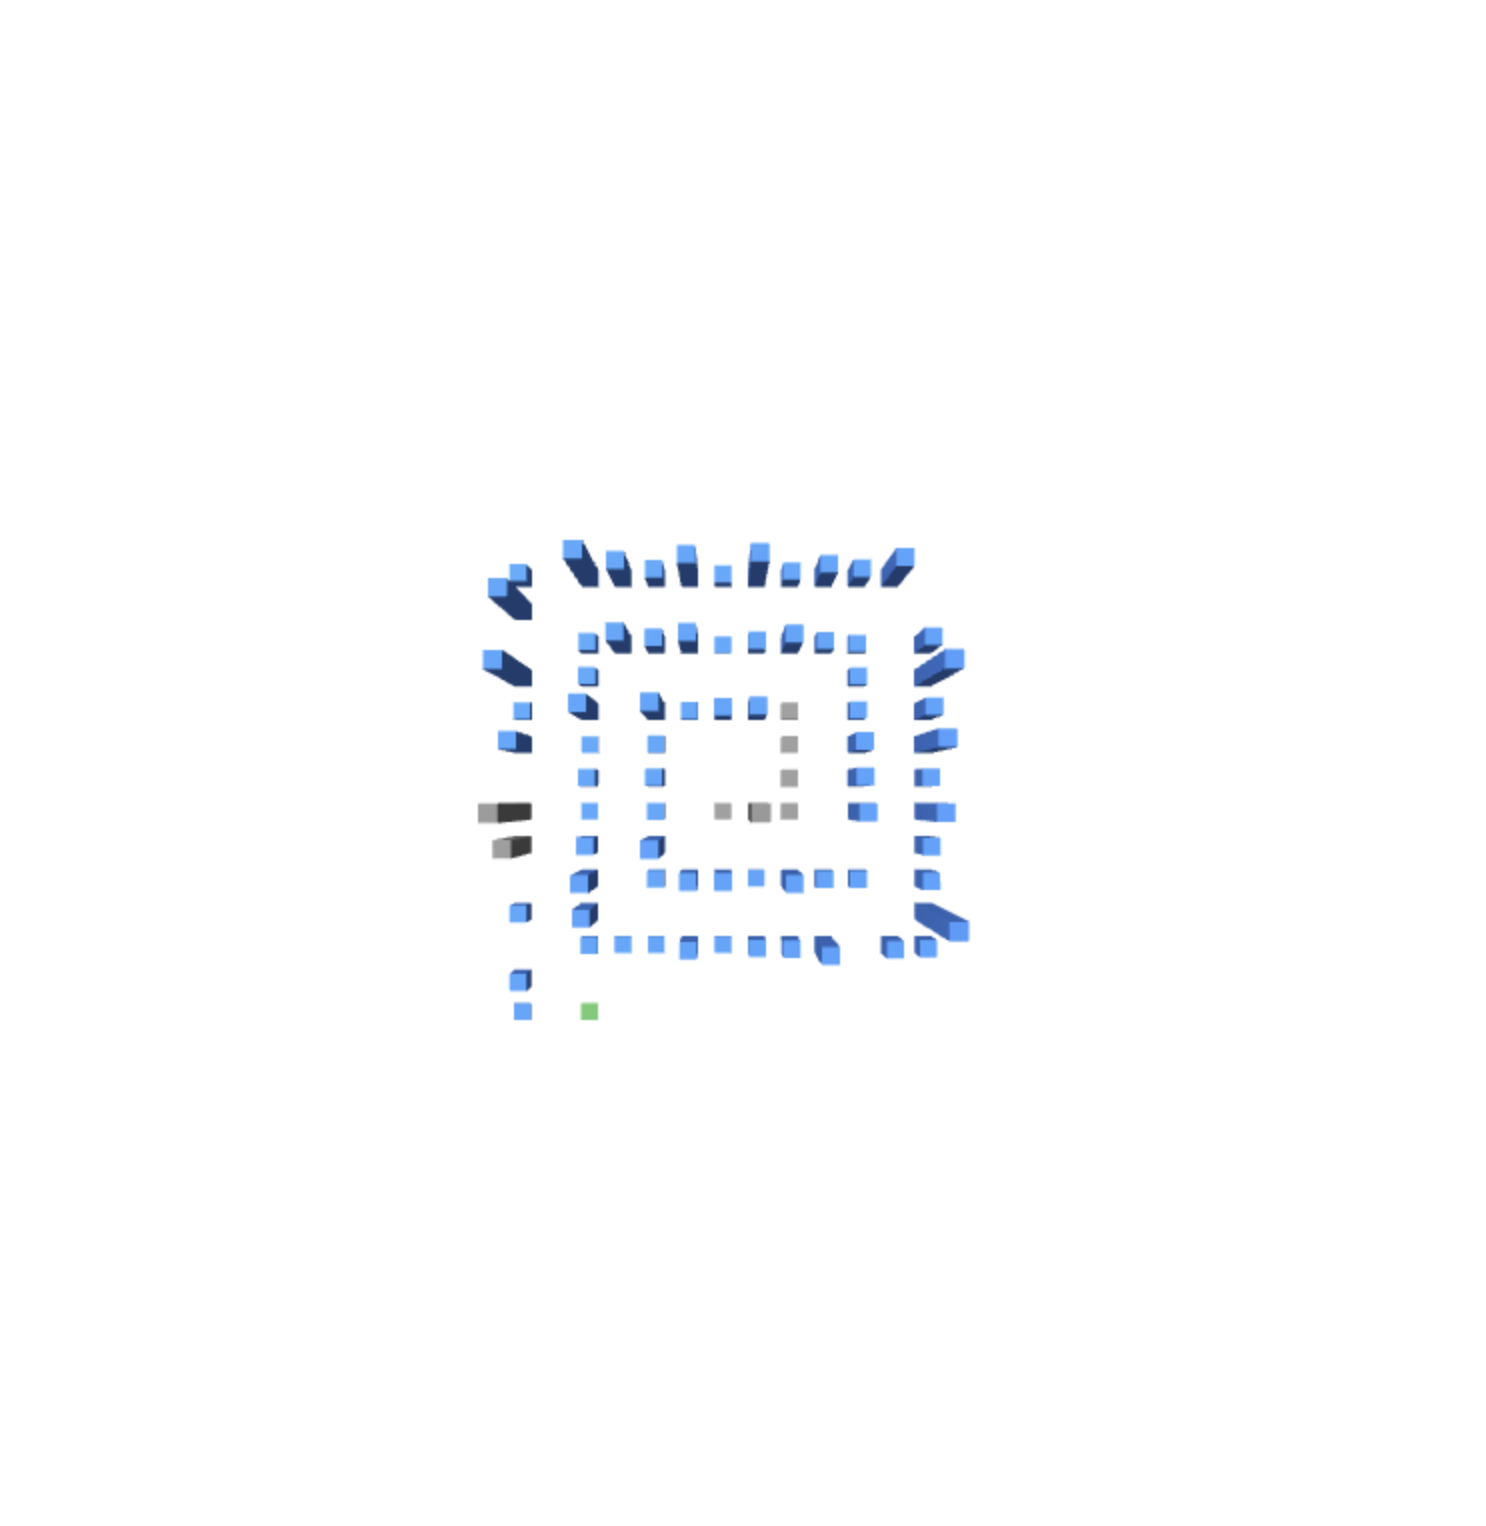
\includegraphics[width=\linewidth]{JetUML_V0S5.png}
        \caption{22 Jan 2015 \linebreak  \#27 Renamed the packages} 
        \label{fig:JetUML_V0S5}
    \end{subfigure}
    \hspace*{\fill}
    \begin{subfigure}{0.32\textwidth}
        
\includegraphics[width=\linewidth]{JetUML_V0S6.png}
        \caption{16 Oct 2015 \linebreak  \#3 New copyright block on ...} 
        \label{fig:JetUML_V0S6}
    \end{subfigure}
    \hspace*{\fill}
    \medskip
    \begin{subfigure}{0.32\textwidth}
        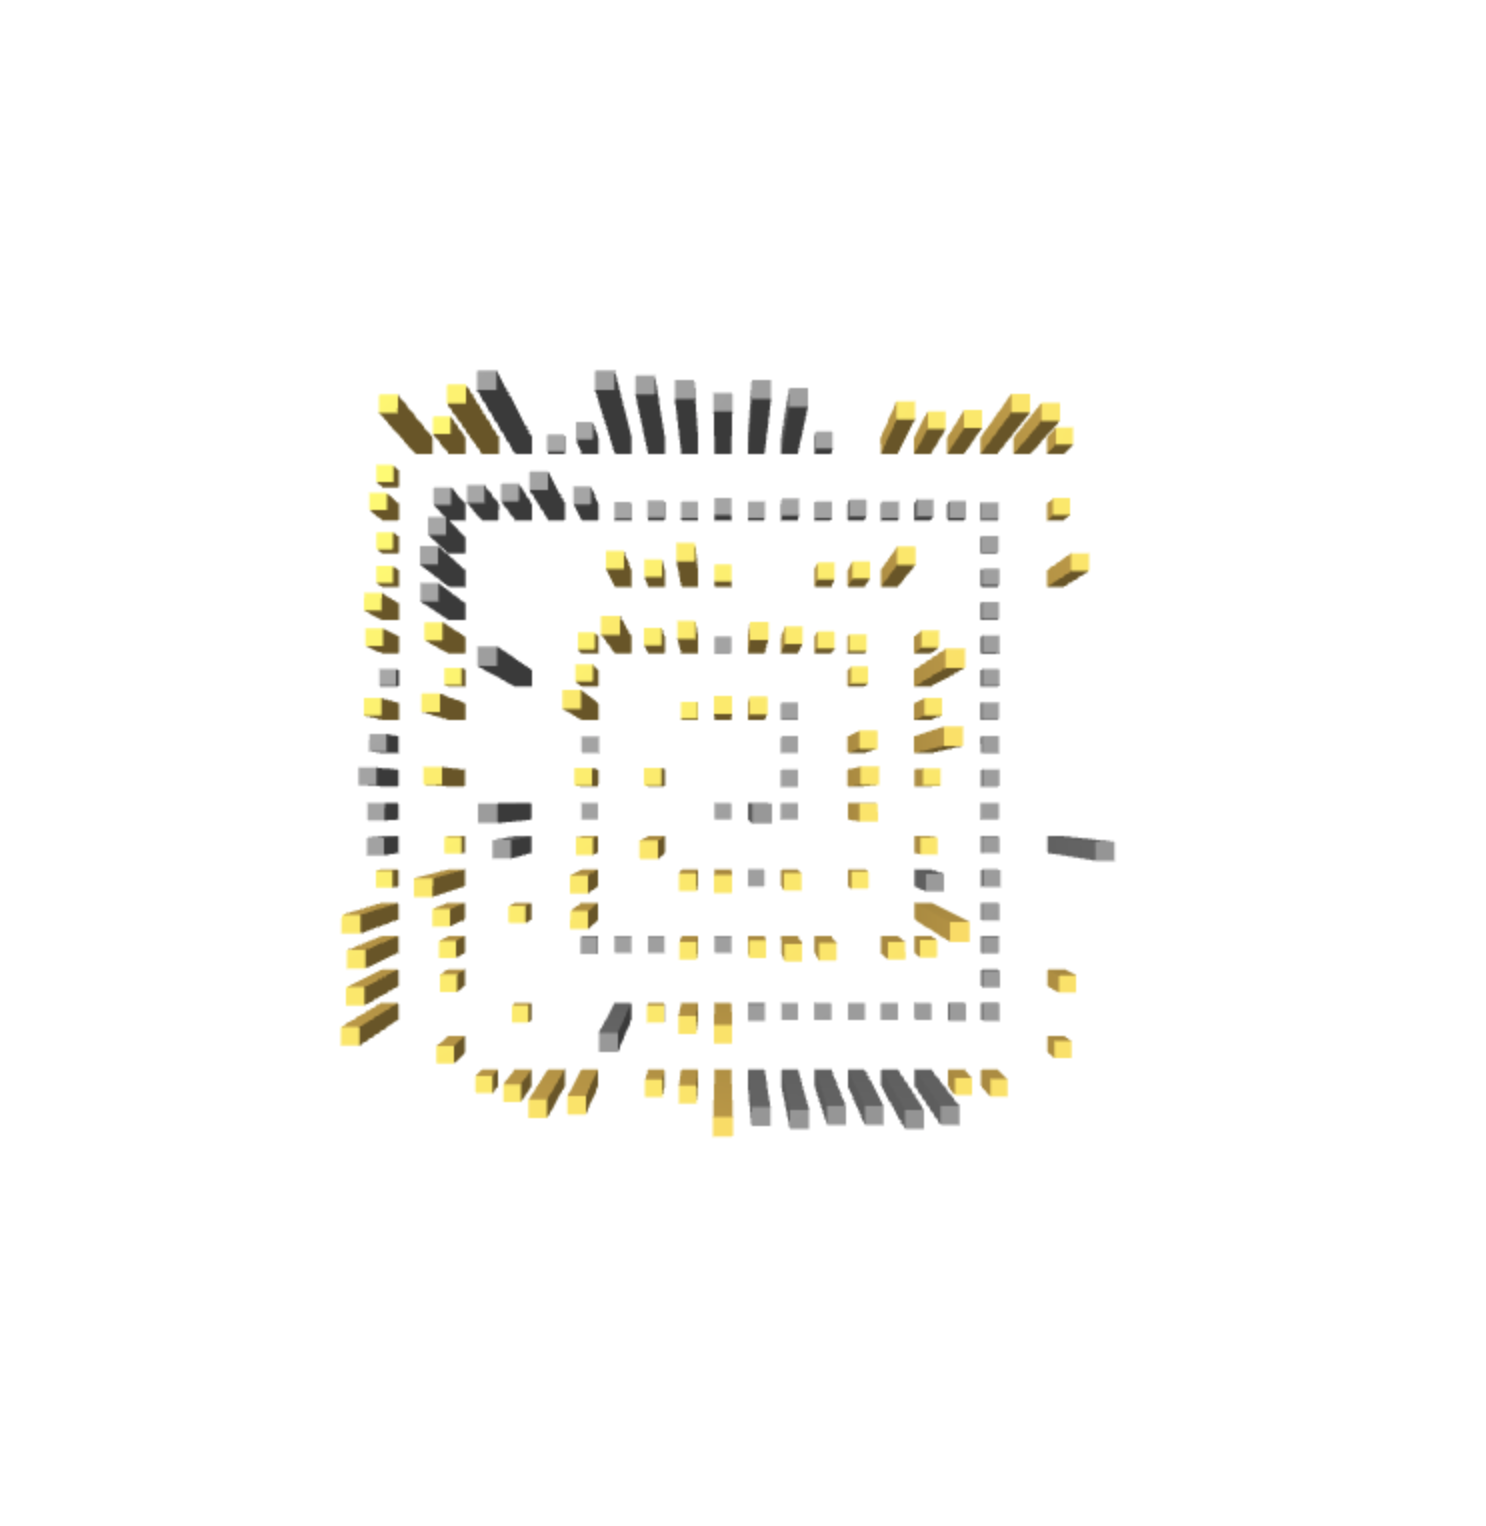
\includegraphics[width=\linewidth]{JetUML_V0S7.png}
        \caption{17 Jan 2016 \linebreak  \#146 Updated the copyright ...}
         \label{fig:JetUML_V0S7}
    \end{subfigure}
    \hspace*{\fill}
    \begin{subfigure}{0.32\textwidth}
        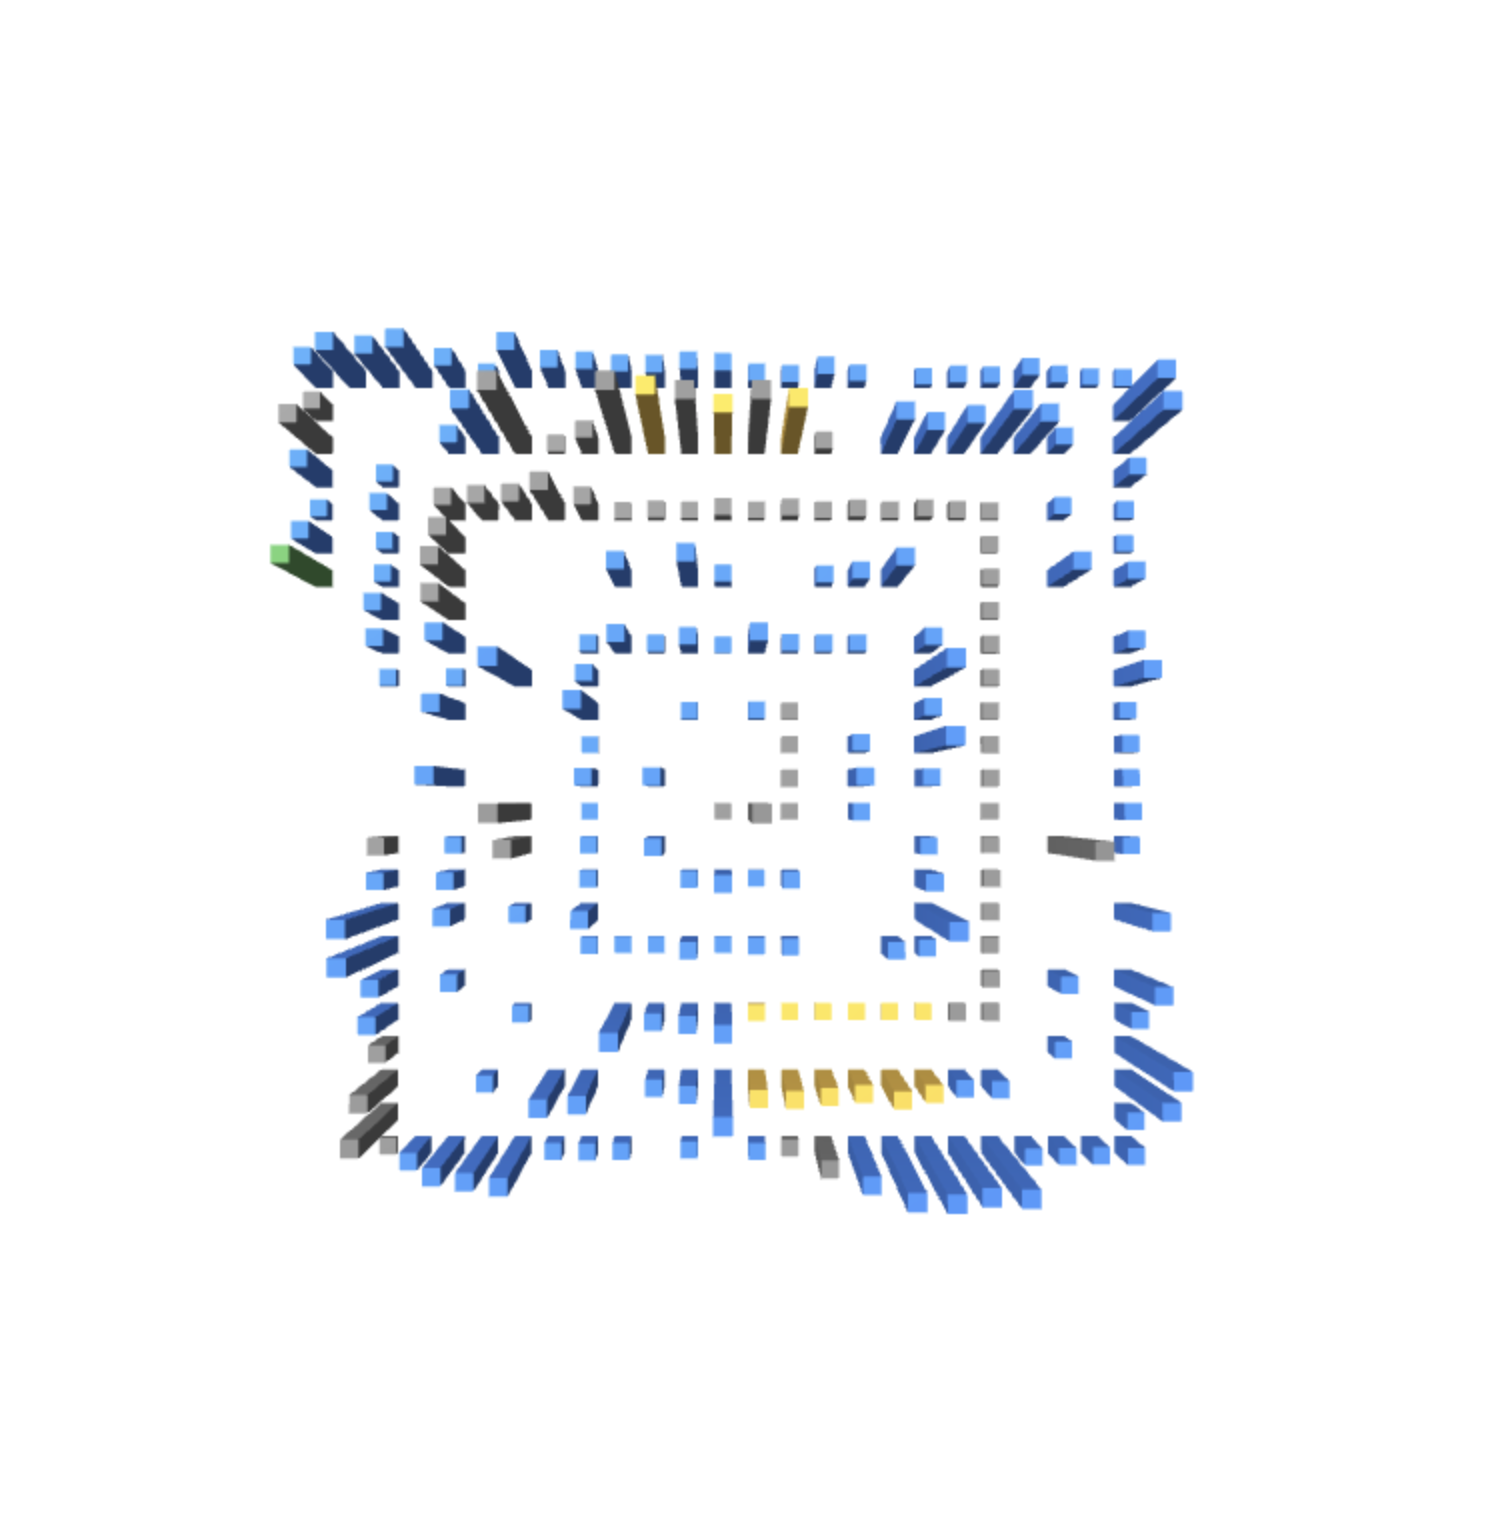
\includegraphics[width=\linewidth]{JetUML_V0S8.png}
        \caption{26 Nov 2017 \linebreak  \#212 Remove stg from name} 
        \label{fig:JetUML_V0S8}
    \end{subfigure}
    \hspace*{\fill}
    \begin{subfigure}{0.32\textwidth}
        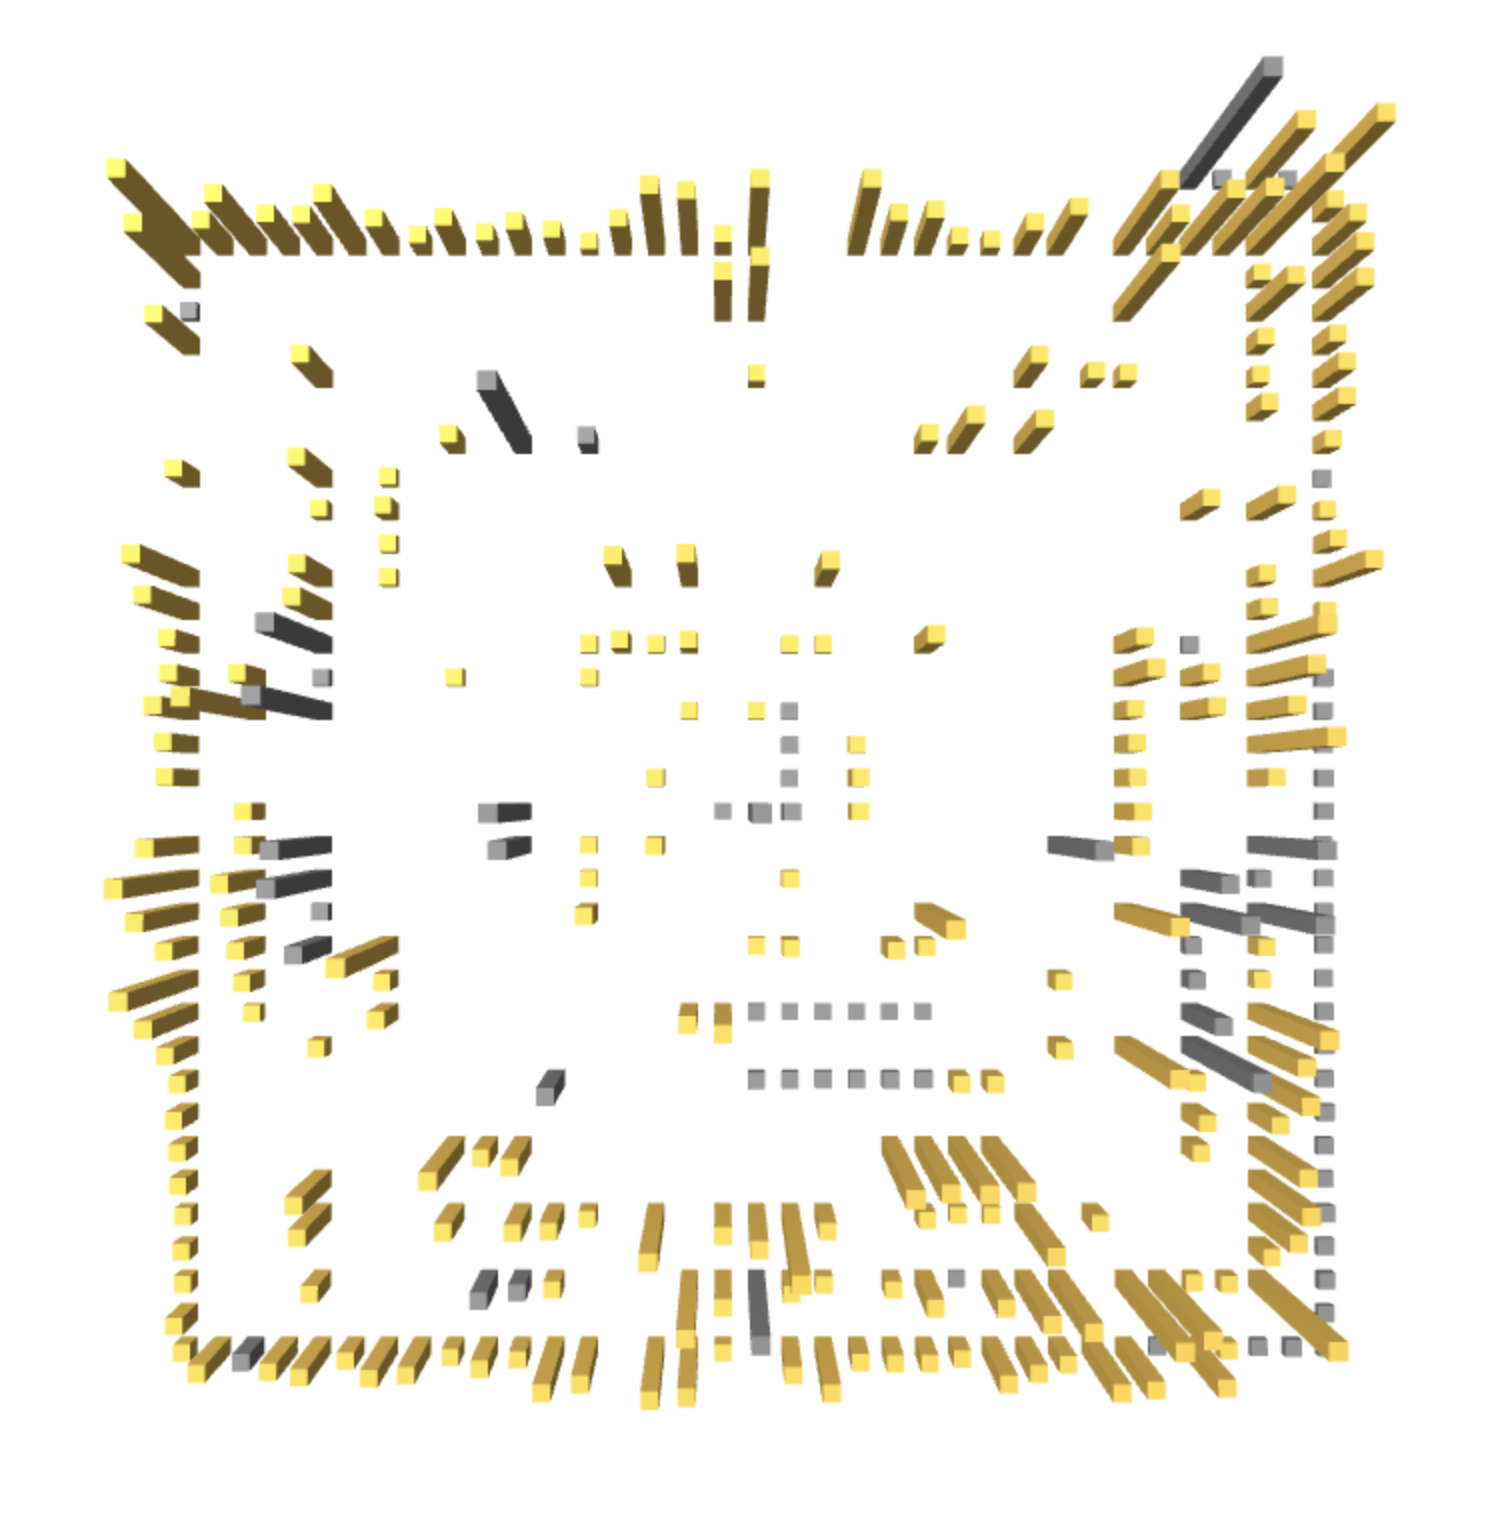
\includegraphics[width=\linewidth]{JetUML_V0S9.png}
        \caption{22 Jul 2020 \linebreak  \#374 Fix copyrights} 
        \label{fig:JetUML_V0S9}
    \end{subfigure}
    \hspace*{\fill}
    \medskip
    \caption{
        Subset of the biggest commits in JetUML. Figure \ref{fig:JetUML_V0S1_3} represent the first commit. In Figure \ref{fig:JetUML_V0S2} they pushed the code of Violetta. Figure \ref{fig:JetUML_V0S3} depicts their first refactoring. In Figure \ref{fig:JetUML_V0S4} they moved some classes from Violet to Violetta. In Figure  \ref{fig:JetUML_V0S5} they moved most of them under JetUML. In Figure \ref{fig:JetUML_V0S6}, \ref{fig:JetUML_V0S7} and \ref{fig:JetUML_V0S9} are depicted three refactoring activities to fix copyrights. In Figure \ref{fig:JetUML_V0S8} most of the entities are painted with blue because they changed their path.} 
    \label{fig:JetUML_V0}
\end{figure}

\subsubsection{View 2}
\textbf{Goal of this visualization}
With this visualization, we want to see how the repository evolved through its first six months. 
The authors of JetUML, during this interval of time, made seven pre-releases of the system. 
Moreover, we want to show what an aging strategy of one month with ten steps looks like. 

\bigbreak
View specification adopted: 
\begin{itemize}
    \item \texttt{versionGroupingStrategy}: timestamp.
    \item \texttt{versionGroupingChunkSize}: 2'629'743 (1 month). 
    \item \texttt{colorPalette}: default.
    \item \texttt{agingGroupingStrategy}: timestamp.
    \item \texttt{agingStepSize}: 2'629'743 (1 month).
    \item \texttt{agingSteps}: 10 steps. 
    \item \texttt{mapperStrategy}: LinearBucketValueStrategy.
    \item \texttt{mapperStrategyOptions}: max height of 20.
    \item \texttt{mapperMetricName}: SIZE. 
    \item \texttt{showUnmappedEntities}: true.
    \item \texttt{fileTypeShape}: all BOX. 
    \item \texttt{fileTypeOpacity}: all 1. 
    \item \texttt{showDeletedEntities}: false.
\end{itemize}

\textbf{Results}
\autoref{fig:JetUML_V1} shows the evolution of JetUML during its first 6 months. \autoref{fig:JetUML_V1S1} shows the state of the repository after its first month. All the entities are painted with the color representing the last action made on that file. All the colors are bright because the age of all the files is set to 0 since the time elapsed between their last action and the last commit of the visualization cannot be higher than one month. The second month is depicted in \autoref{fig:JetUML_V1S2}. Here we can easily spot older entities as they are darker than others. This means that some files had not been touched since the first month at the end of the second month. In the third and the fourth month, more or less the same amount of files was updated. However, in the fifth month, only three entities were modified; consequently, all the others are darker because they are older. 
At the end of the sixth month, two entities were added and modified. However, most of the entities were still getting older. 

\textbf{Conclusion}
We have seen how different is the timestamp strategy compared to what we saw in the first visualization. Here, the number of frames does not depend upon the number of commits made; instead, it relies on the number of months part of the history. 
However, the choice of the aging strategy also played a crucial role in this visualization. It highlighted updated entities without hiding the last action made on the others. Looking at \autoref{fig:JetUML_V1S6} we can immediately see that many files were added and never touched because their color looks dark green. The cause of this inactivity on the file may be related to the file type, and this limits our visualization because we cannot infer the type in any way. 


% With this visualization, we want to see how all JetUML files evolved through time. 
% JetUML does not seem to have a fixed release cycle.
% Since its history spans eight years of activity; we initially chose a timestamp grouping strategy of one month. 
% As a consequence, we have 89 AnimationFrames. 
% In this first visualization, we do not care about the FileType of entities; we are interested in all of them. 
% Grouping commits monthly; we applied the same strategy to the aging to see how many months had passed since an entity was modified. 
% To summarize, the view specification of this visualization is the following:

% Figure \ref{fig:JetUML_V1} shows the first 6 month of evolution of JetUML. 
% We can infer many things by looking at these figures. In figure \ref{fig:JetUML_V1S1} 7 entities have been moved. 
% Most of them are files with the extension \texttt{.properties}, and perhaps they were involved in a refactoring activity since their path changed from
% \texttt{src/ca/mcgill/cs/stg/jetuml/...} to \texttt{src/ca/mcgill/cs/stg/jetuml/diagrams/...}. 
% At the end of their first month of activity, they had 135 files and made 127 commits. 
% We can see many files are still green. This means that they were added but never touched after. 
% An issue with this visualization is that we cannot distinguish Java files from others. 
% These added files are images. Therefore it is not a surprise that once added; they are never modified in the future. 
% In figure \ref{fig:JetUML_V1S2} where the second month is represented, we can see that some entities have a darker color. 
% This means that during the second month, they were not touched. 
% Comparing all the figures until figure \ref{fig:JetUML_V1S6} we can notice that many entities have the same behavior. 
% They were added and updated in the first month of activity (this is why they are yellow), and then they were never touched, becoming darker and darker each month. 

\begin{figure}[h!]
    \begin{subfigure}{0.48\textwidth}
    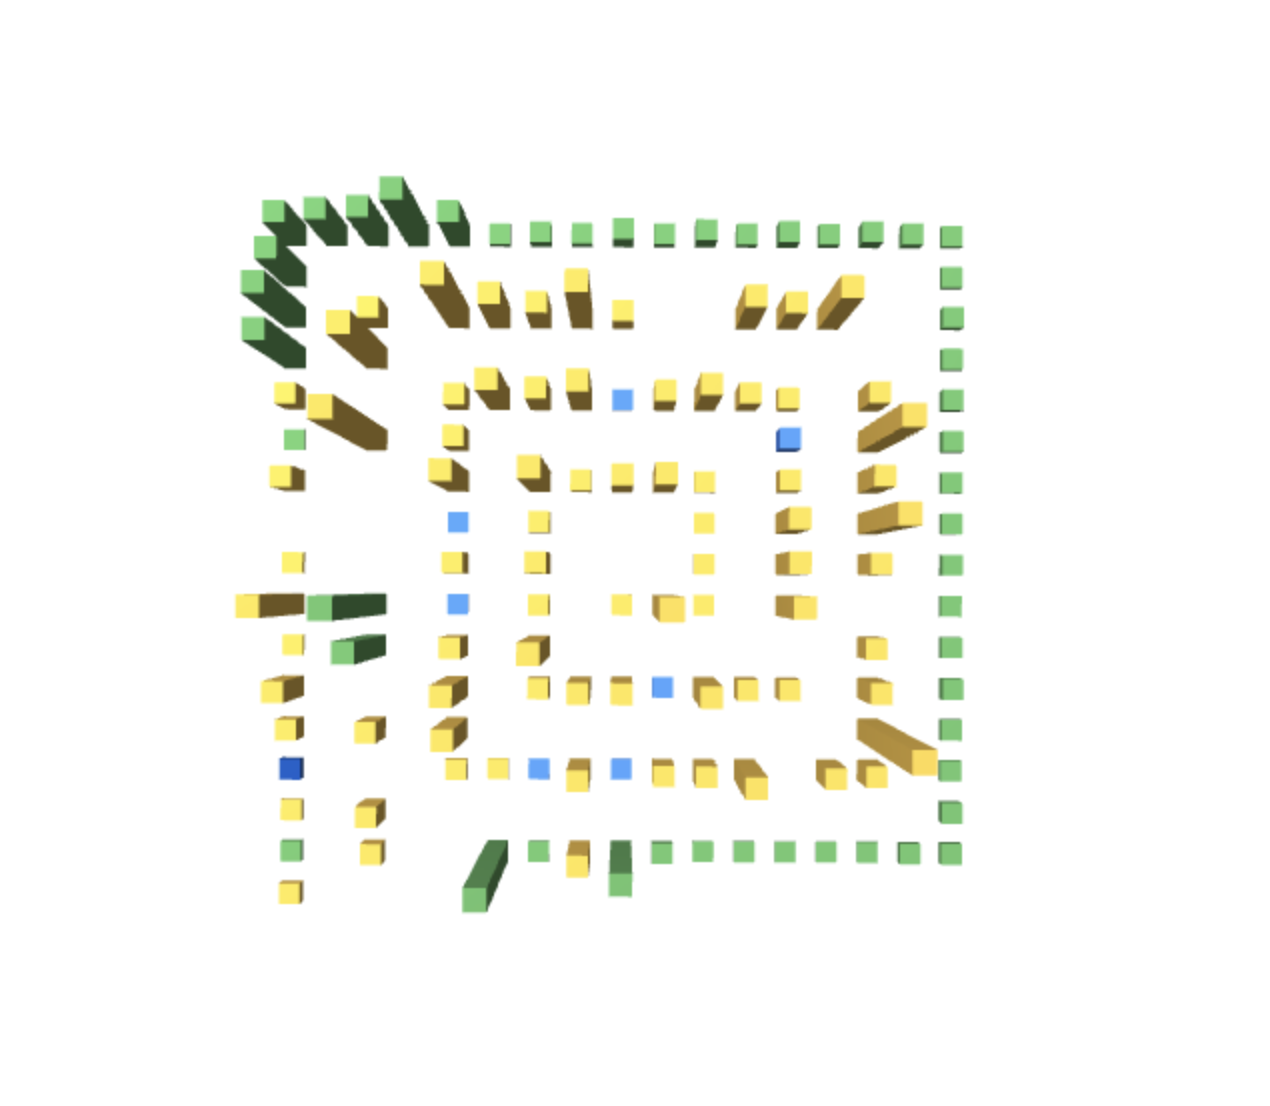
\includegraphics[width=\linewidth]{JetUML_V1S1.png}
    \caption{Month 1} \label{fig:JetUML_V1S1}
    \end{subfigure}\hspace*{\fill}
    \begin{subfigure}{0.48\textwidth}
        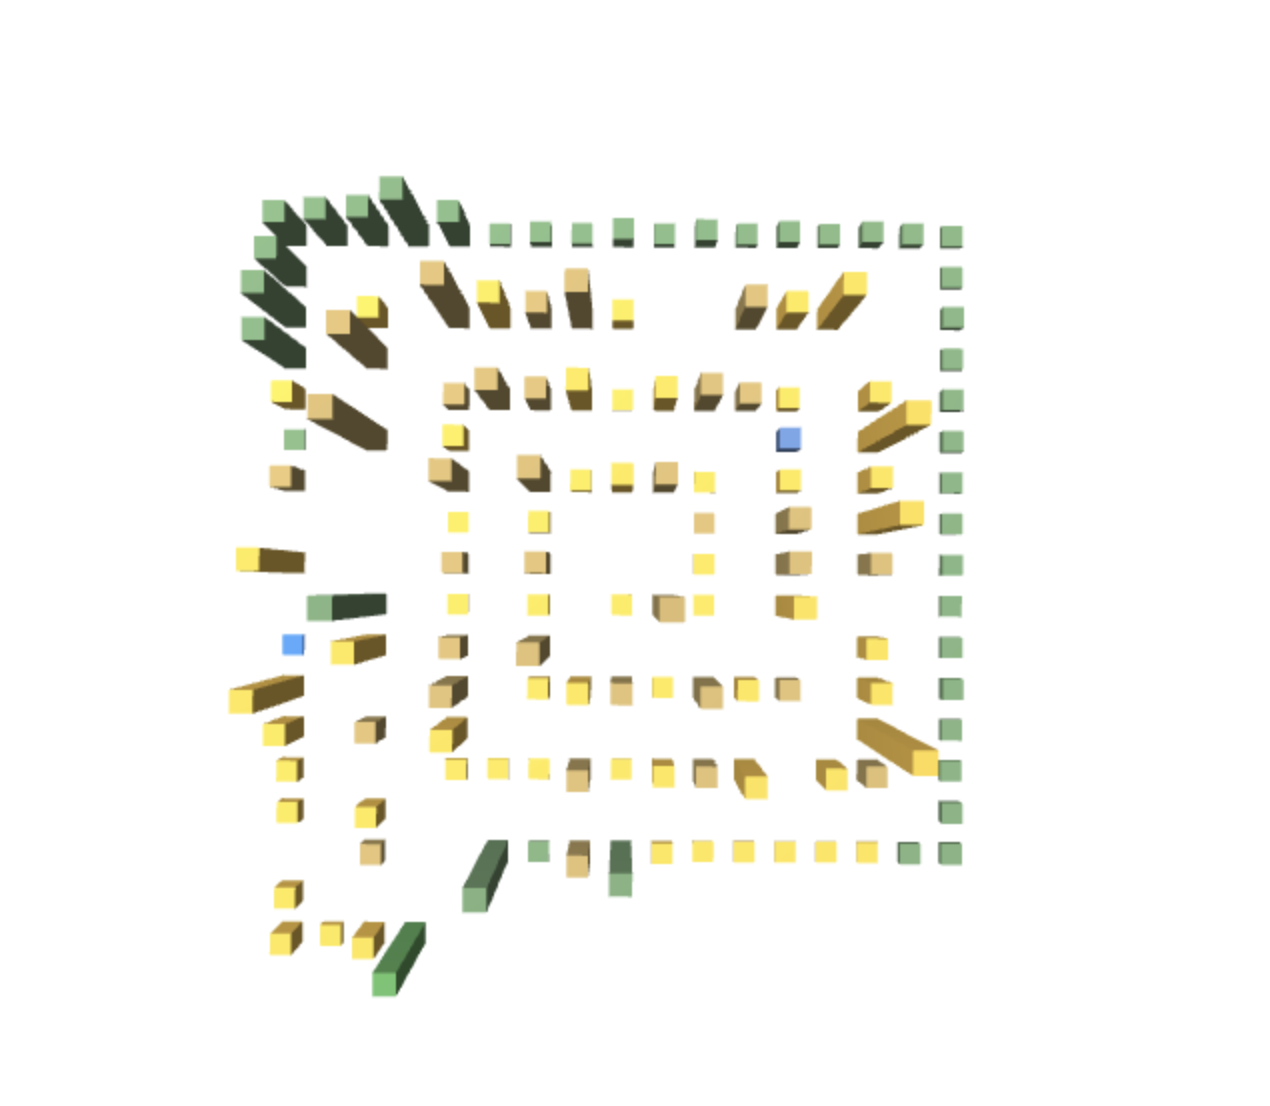
\includegraphics[width=\linewidth]{JetUML_V1S2.png}
        \caption{Month 2} \label{fig:JetUML_V1S2}
    \end{subfigure}
    
    \medskip
    \begin{subfigure}{0.48\textwidth}
        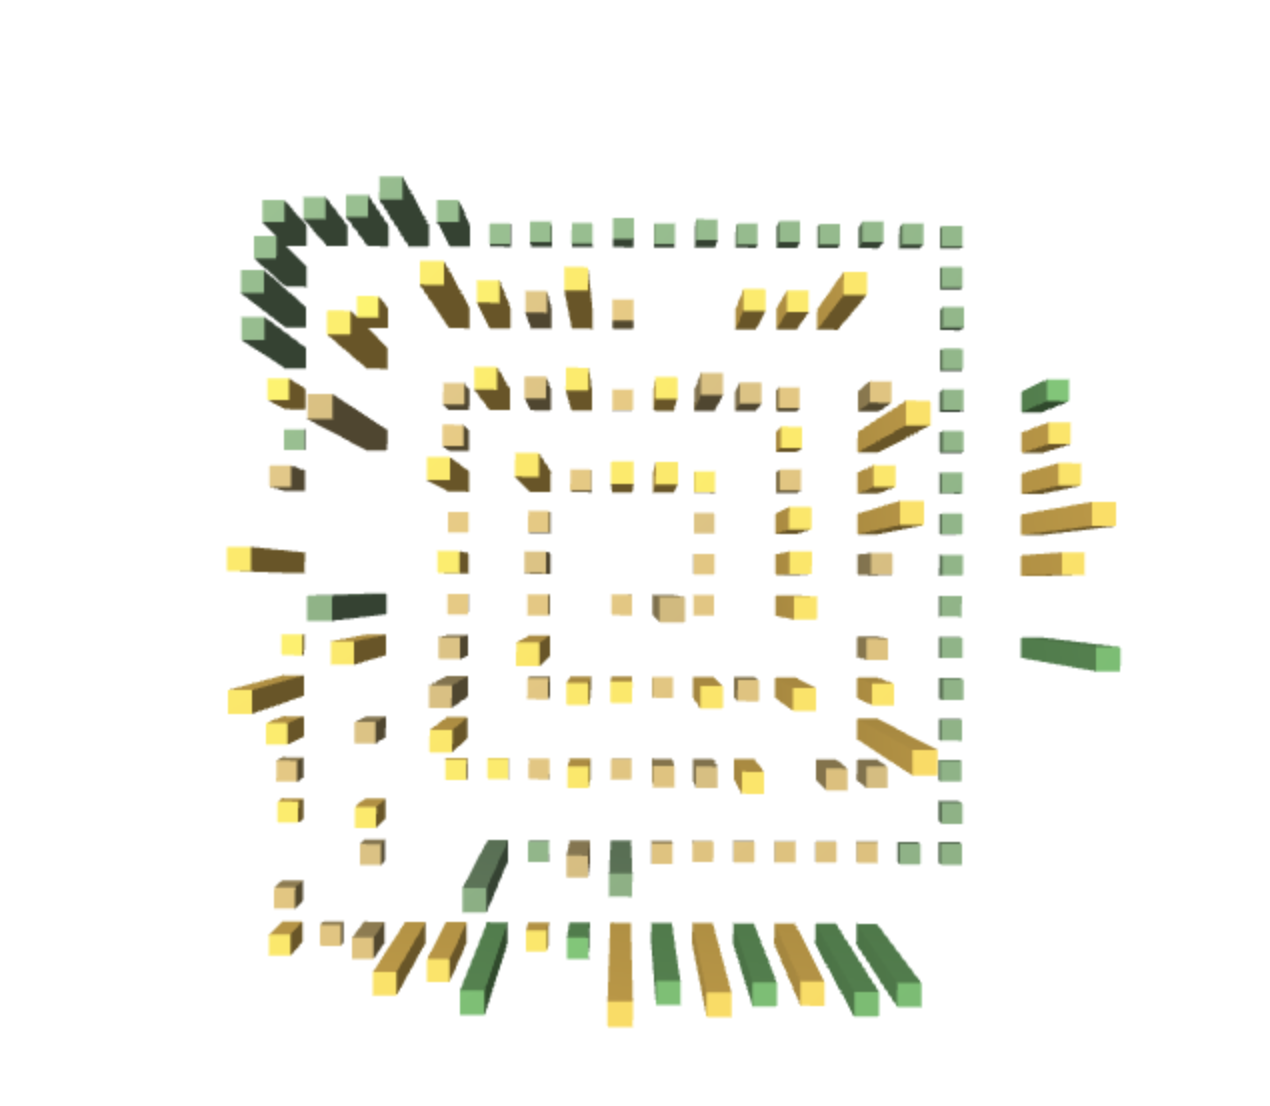
\includegraphics[width=\linewidth]{JetUML_V1S3.png}
        \caption{Month 3} \label{fig:JetUML_V1S3}
    \end{subfigure}\hspace*{\fill}
    \begin{subfigure}{0.48\textwidth}
    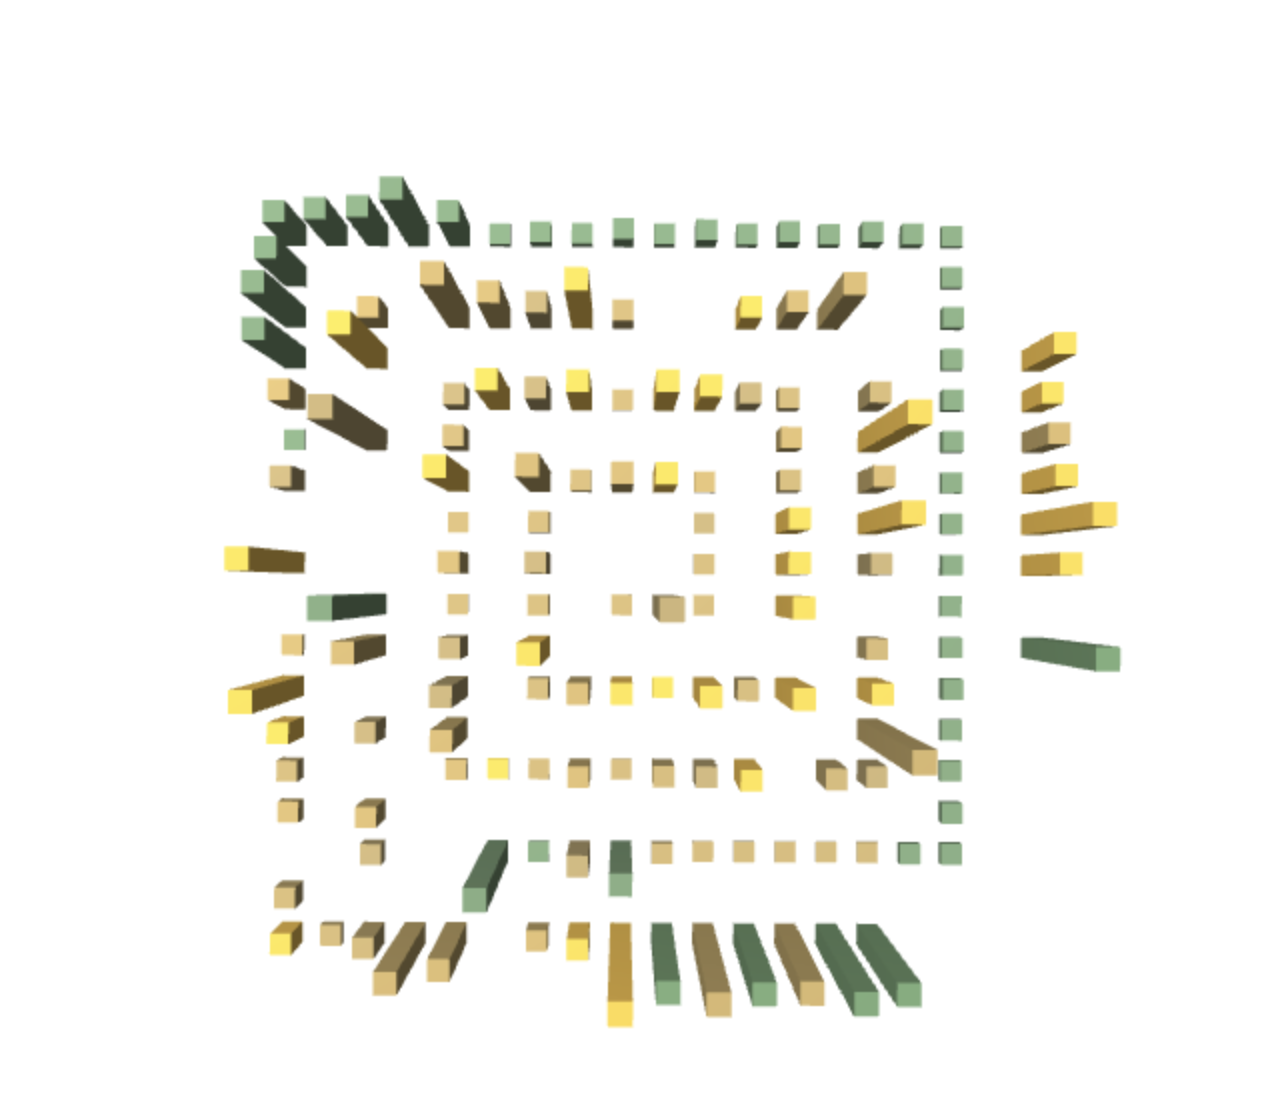
\includegraphics[width=\linewidth]{JetUML_V1S4.png}
    \caption{Month 4} \label{fig:JetUML_V1S4}
    \end{subfigure}
    
    \medskip
    \begin{subfigure}{0.48\textwidth}
        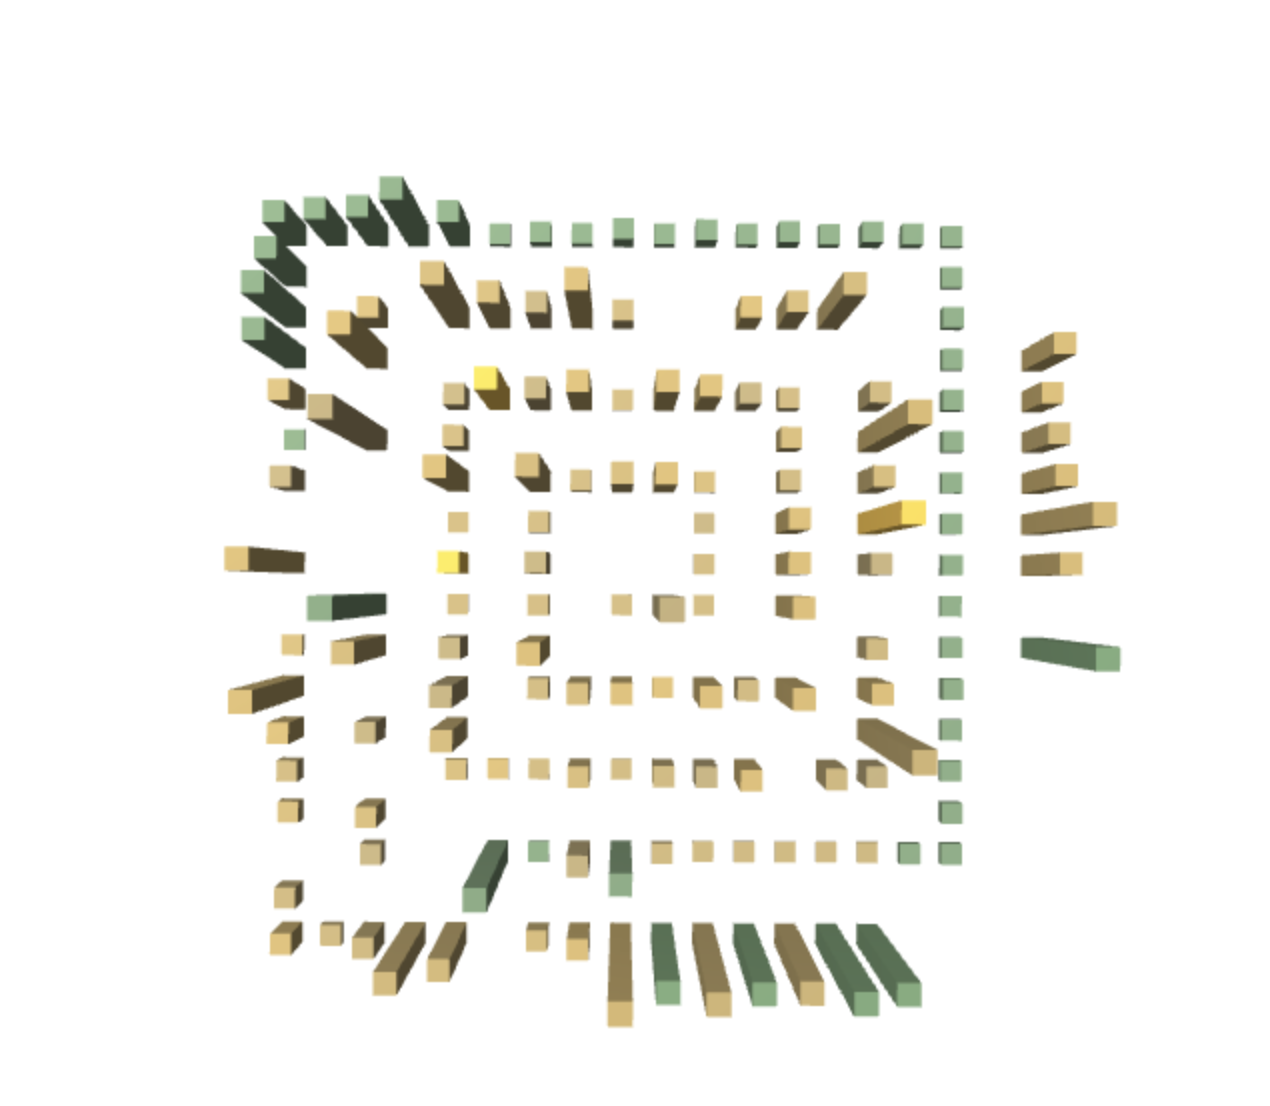
\includegraphics[width=\linewidth]{JetUML_V1S5.png}
        \caption{Month 5} \label{fig:JetUML_V1S5}
    \end{subfigure}\hspace*{\fill}
    \begin{subfigure}{0.48\textwidth}
        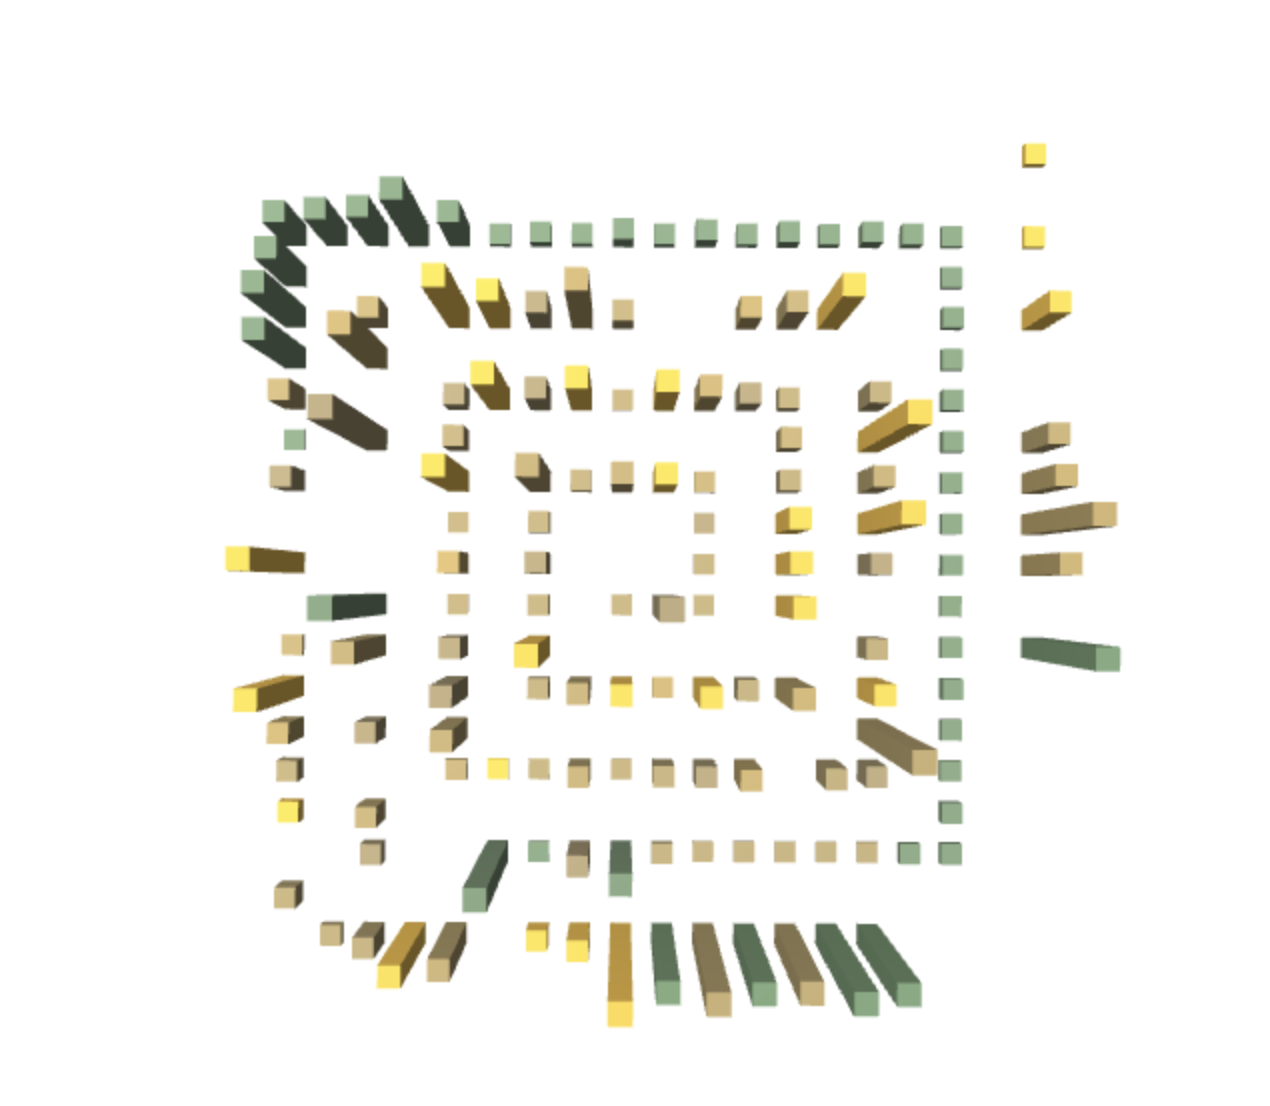
\includegraphics[width=\linewidth]{JetUML_V1S6.png}
        \caption{Month 6} \label{fig:JetUML_V1S6}
    \end{subfigure}
    
    \caption{First six month of the JetUML evolution.} 
    \label{fig:JetUML_V1}
\end{figure}
\subsubsection{View 3}
\textbf{Goal of this visualization}
In this third and last visualization that we propose, the goal is to study the entire evolution of the system, with a focus on Java files. 
To do that, the use the shape and opacity property of a ViewFigure, to distinguish them among others. 
To display the evoluition of the system we adopt a timestamp grouping strategy, with a timestamp of one year. 
Furthermore, we also adop a timestamp strategy for the aging, with a total of ten steps and a time window of one month. This means that grey entities represent files that have not been received any update for the last 10 month from the time of the displayed AnimationFrame. 
\begin{itemize}
    \item \texttt{versionGroupingStrategy}: timestamp.
    \item \texttt{versionGroupingChunkSize}: 31'556'926 (1 year). 
    \item \texttt{colorPalette}: default.
    \item \texttt{agingGroupingStrategy}: timestamp.
    \item \texttt{agingStepSize}: 2'629'743 (1 month).
    \item \texttt{agingSteps}: 10 steps. 
    \item \texttt{mapperStrategy}: LinearBucketValueStrategy.
    \item \texttt{mapperStrategyOptions}: max height of 20.
    \item \texttt{mapperMetricName}: SLOC. 
    \item \texttt{showUnmappedEntities}: true.
    \item \texttt{fileTypeShape}: Java -> BOX, OTHERS -> SPHERE. 
    \item \texttt{fileTypeOpacity}: Java -> max, OTHERS -> low. 
    \item \texttt{showDeletedEntities}: false.
\end{itemize}

\textbf{Results}
The whole evolution of JetUML is depicted in \autoref{fig:JetUML_V3}. As we can notice, it is straightforward to distinguish java files from others because they have different shapes and other files are more transparent. After the first year of development, the state of the repository is shown in \autoref{fig:JetUML_V3S1}. We notice that all the Java files have more or less the same age. This means that all of them were updated after the second month because otherwise, they would be grey. The system grew at the end of the second year, shown in figure \autoref{fig:JetUML_V3S2} and now we can see some grey entities. Most of them are in the middle, meaning that the "core" files, or the files added before others, were not touched after the fourteenth month.  \autoref{fig:JetUML_V3S3} shows the state of the repository at the end of the third year. The system grew, and all the Java files were updated recently. Considering what we have seen in the first visualization, they had to change the path from all the Java files (\autoref{fig:JetUML_V0S8}). Perhaps this can be the reason why all the entities were updated, and some ViewFigures are painted with the blue color. The fourth year of development, shown in  \autoref{fig:JetUML_V3S4}, recorded a little activity in the first months because the system grew, and almost all the entities have a different color. However, it tends to be close to the base color, meaning they are old. 
\autoref{fig:JetUML_V3S5},  \autoref{fig:JetUML_V3S6} and  \autoref{fig:JetUML_V3S7} shows how the system evolved through the fifth, sixth and seventh year. The fifth year recorded an intense activity compared to what we saw in the fourth year. Lots of files were added, and most of the classes of the system were modified. Moreover, the system's center is slowly disappearing, meaning that new ones have replaced old Java files. In the sixth and seventh years, non-Java files were added, and some Java classes were updated outside the system's core. Finally, the last year, represented by \autoref{fig:JetUML_V3S8}, did not record such a huge activity on the system. It became inactive since almost all the entities are grey, meaning that these files were not touched in the last ten months of evolution. However, in this frame, the two tallest entities of the repository exist. This means that in this last year, two java files were added (they were not present the year before), and they rapidly became the biggest files in the system.  

\textbf{Conclusion}
With this visualization, we have seen JetUML from another point of view. The year visualization works very well with systems like JetUML with a comprehensive history. In fact, with just 8 AnimationFrames, we can infer when the development process was more intense in the past. 


\begin{figure}[h!]
    \begin{subfigure}{0.50\textwidth}
        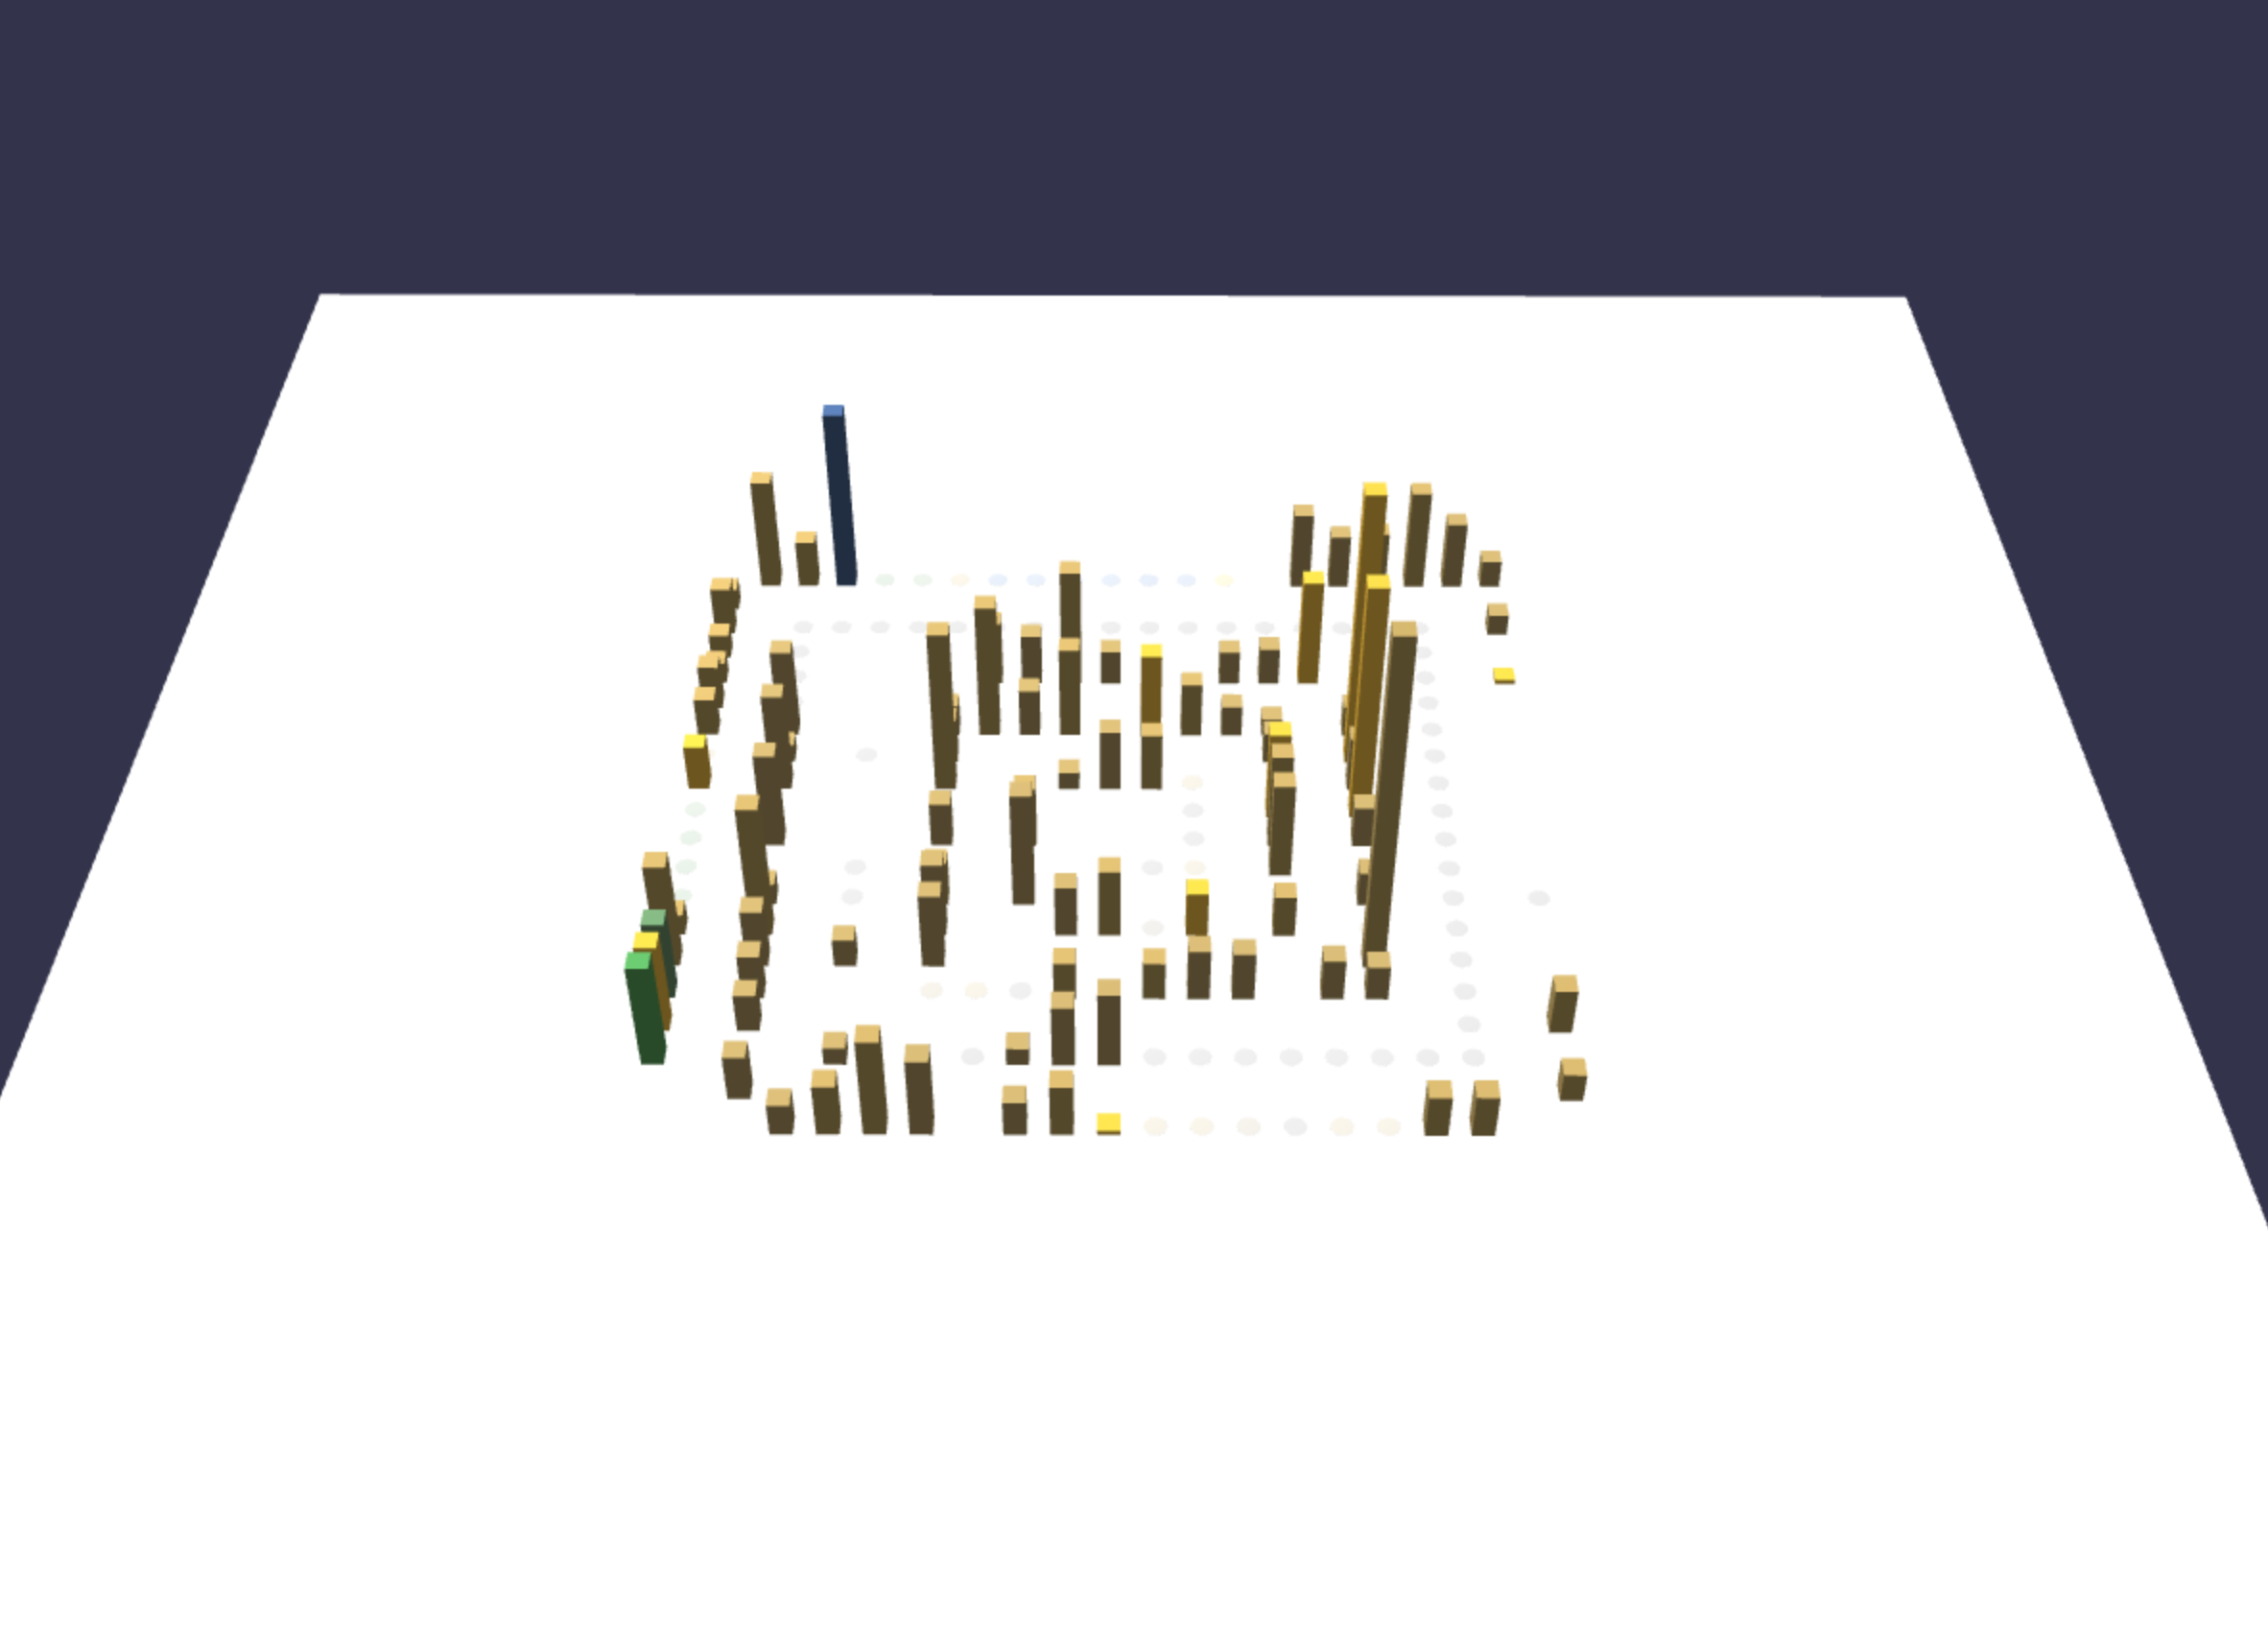
\includegraphics[width=\linewidth]{JetUML_V3S1.png}
        \caption{Year 1} 
        \label{fig:JetUML_V3S1}
    \end{subfigure}\hspace*{\fill}
    \begin{subfigure}{0.50\textwidth}
        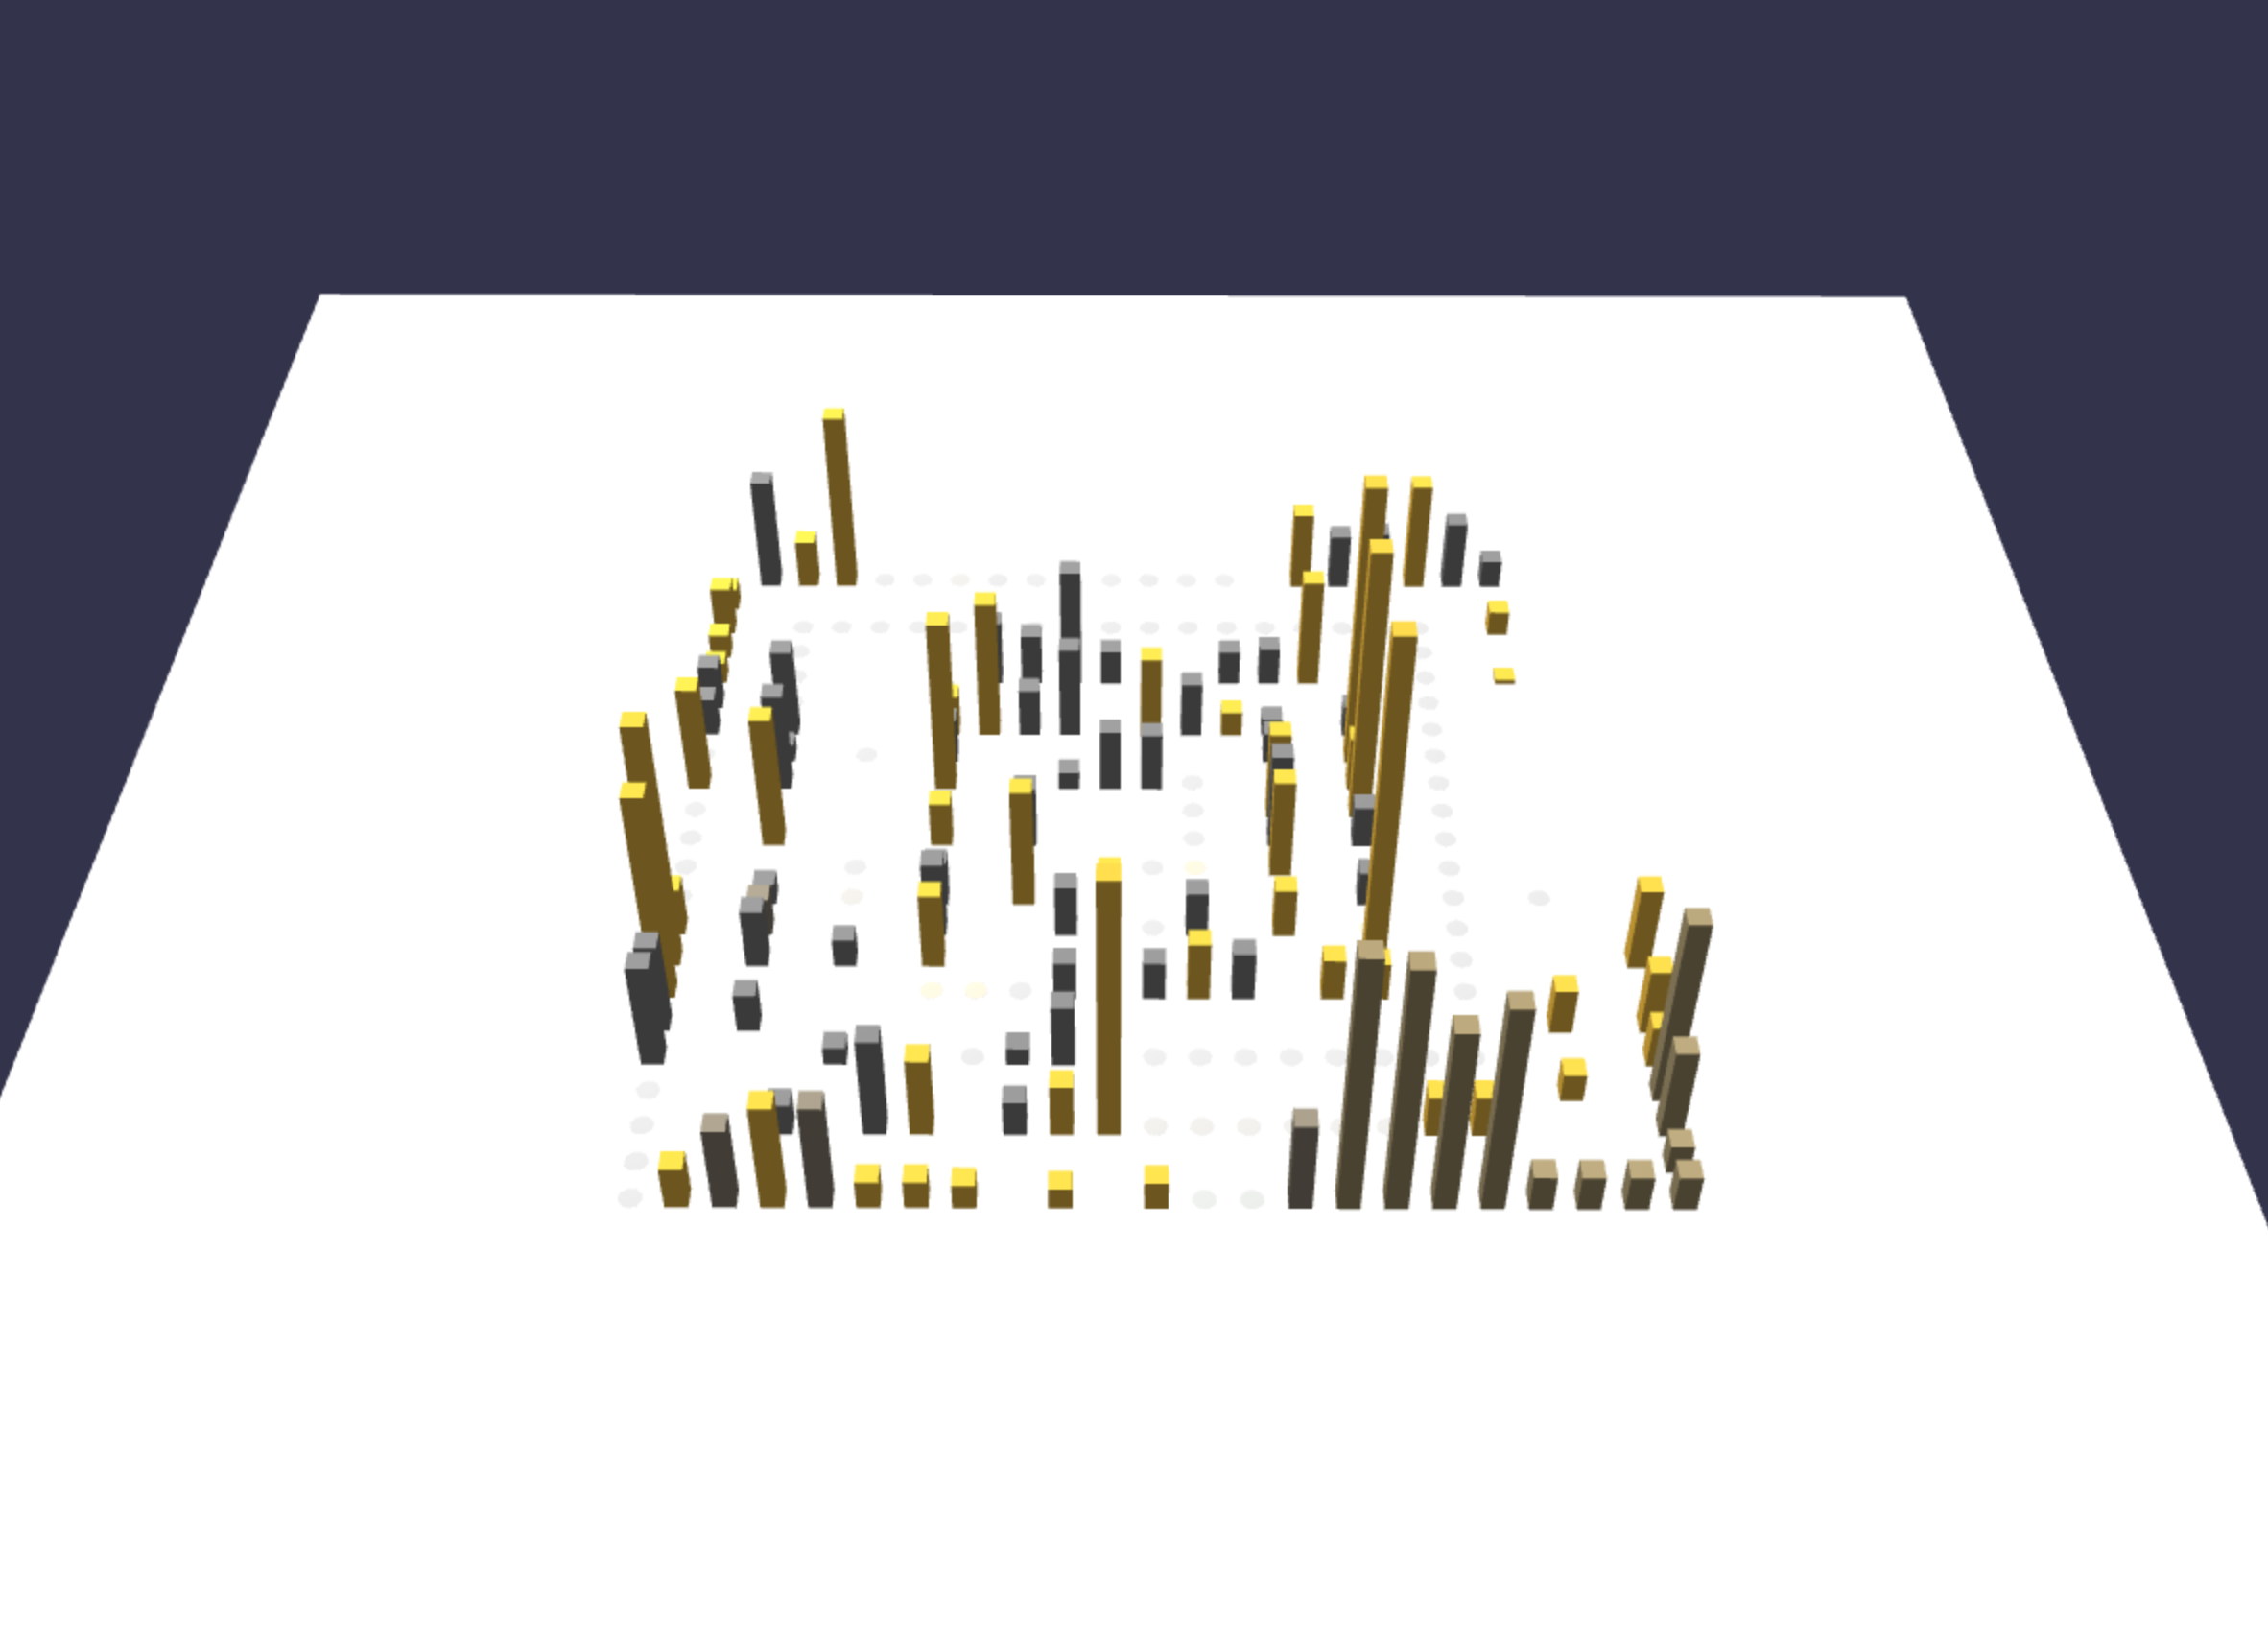
\includegraphics[width=\linewidth]{JetUML_V3S2.png}
        \caption{Year 2} 
        \label{fig:JetUML_V3S2}
    \end{subfigure}
    
    \medskip
    \begin{subfigure}{0.48\textwidth}
        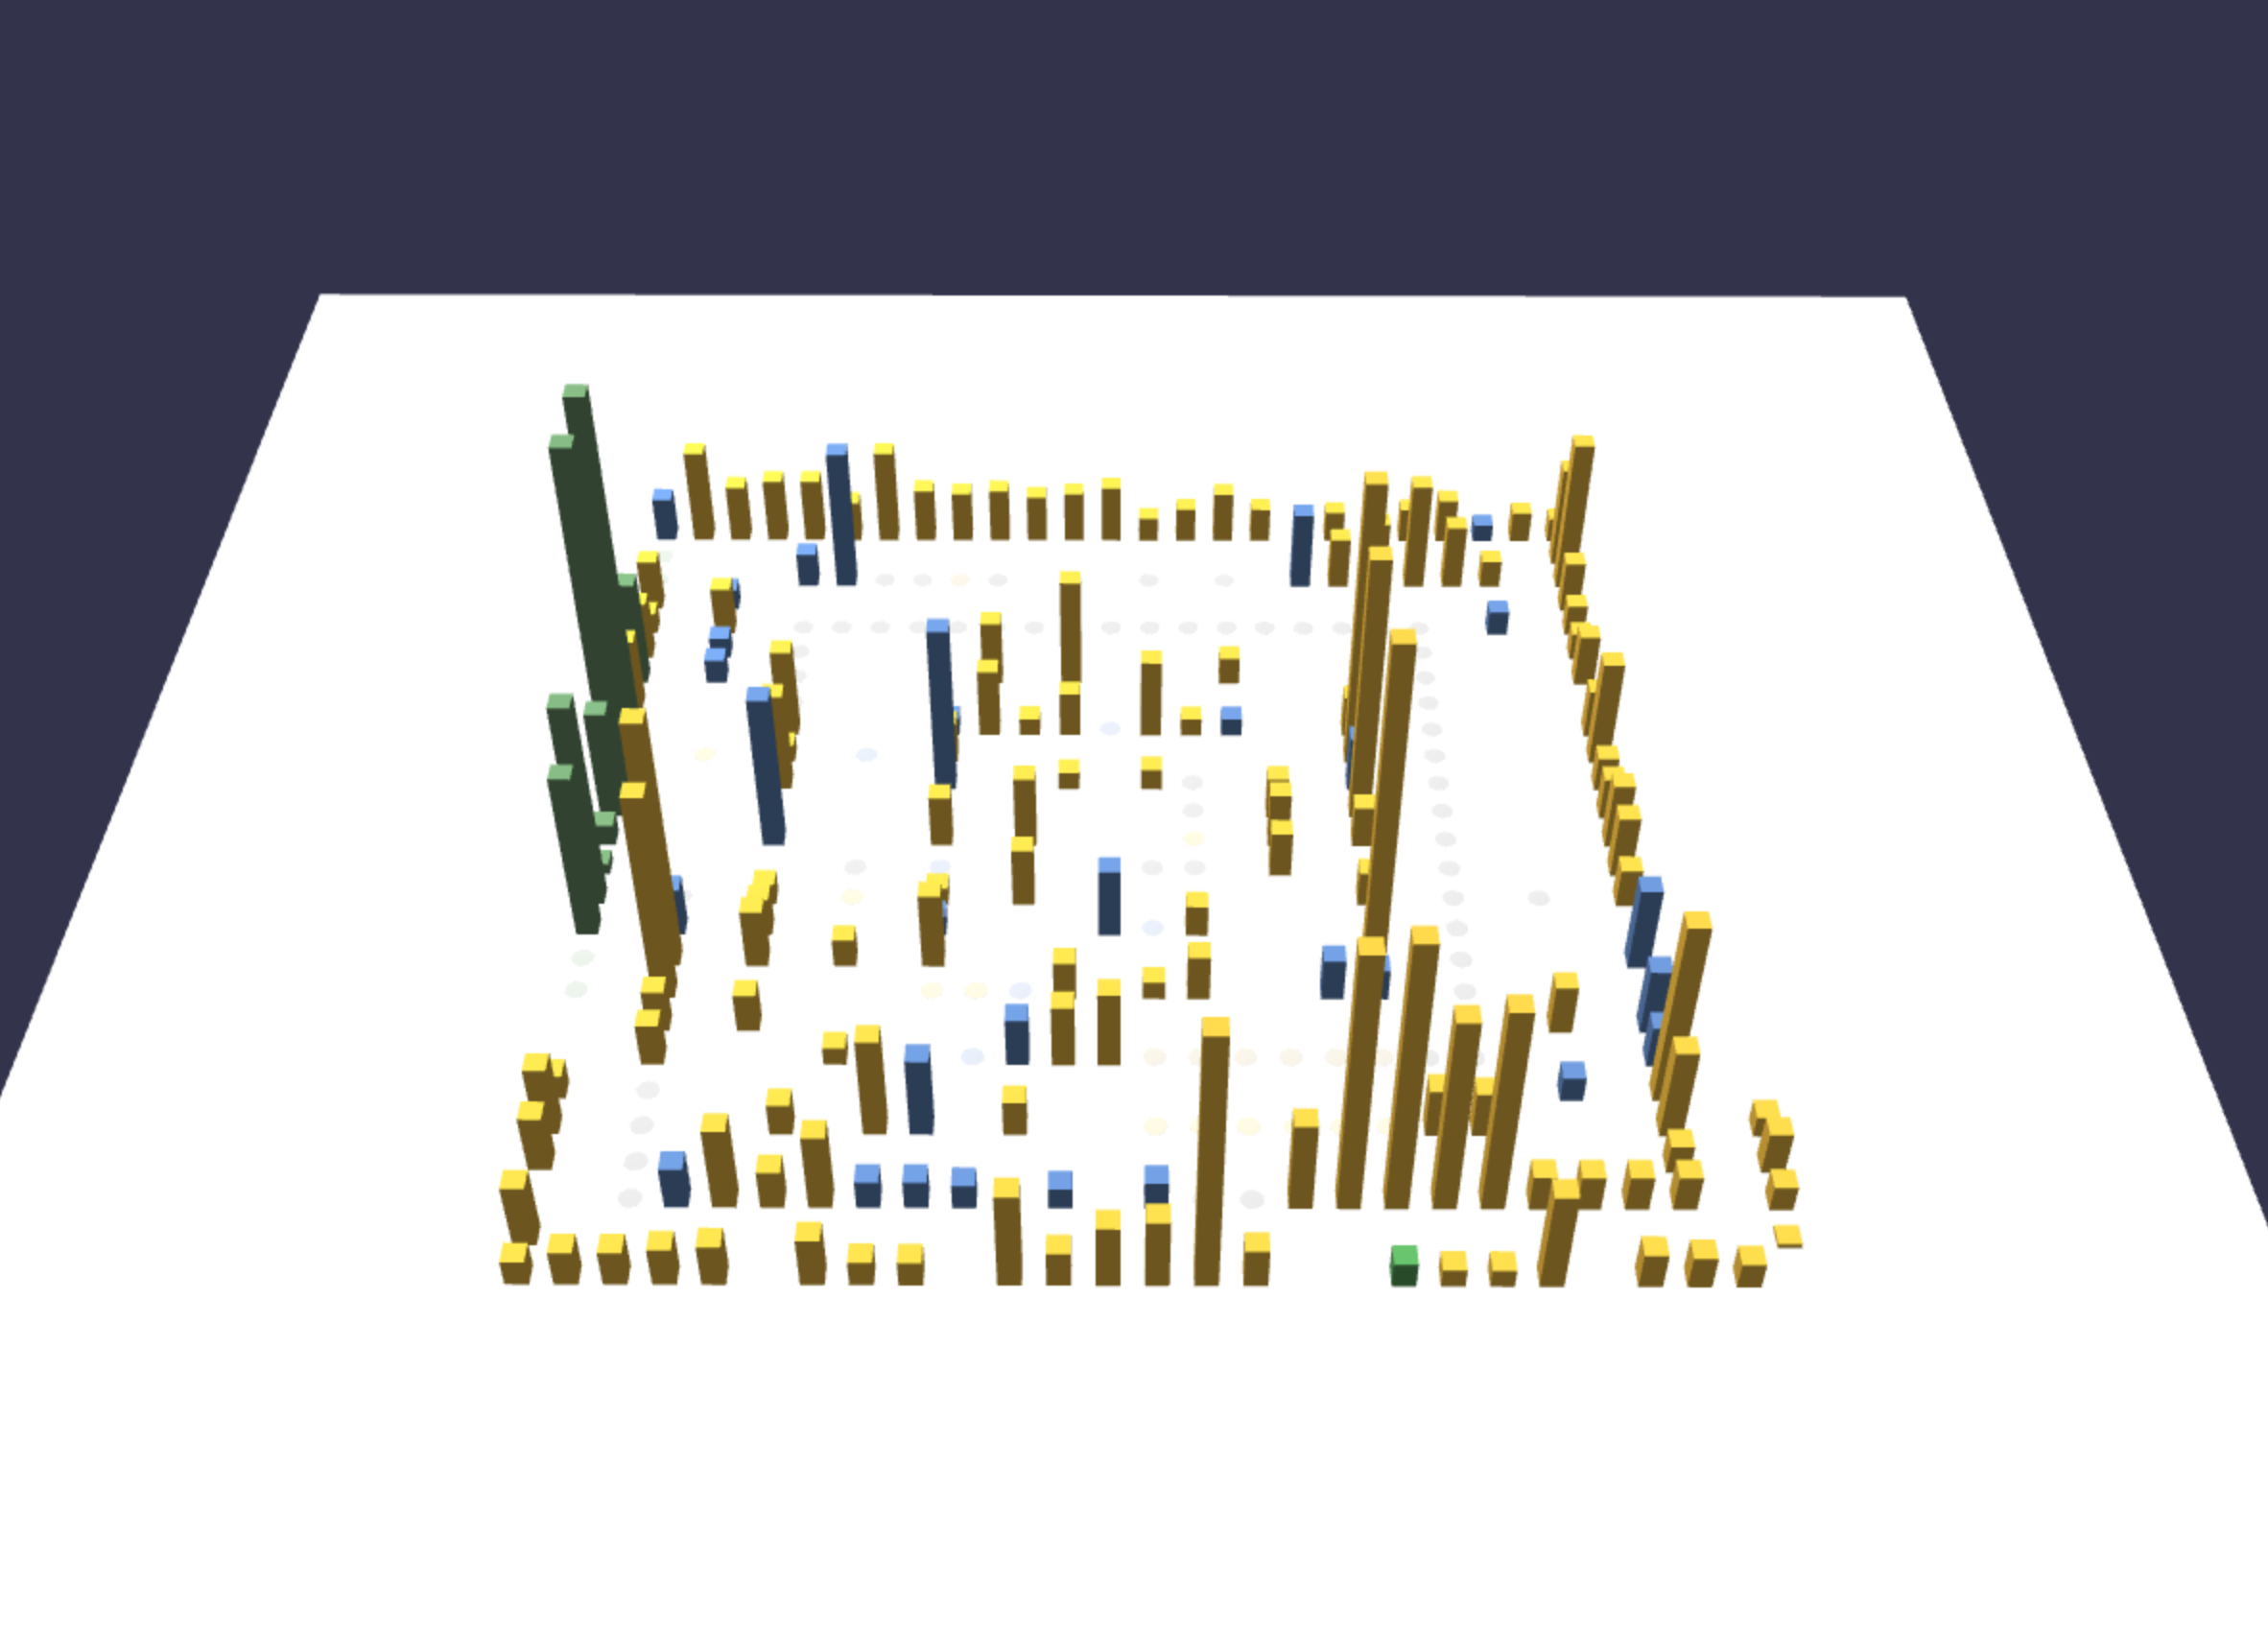
\includegraphics[width=\linewidth]{JetUML_V3S3.png}
        \caption{Year 3} 
        \label{fig:JetUML_V3S3}
    \end{subfigure}\hspace*{\fill}
    \begin{subfigure}{0.48\textwidth}
        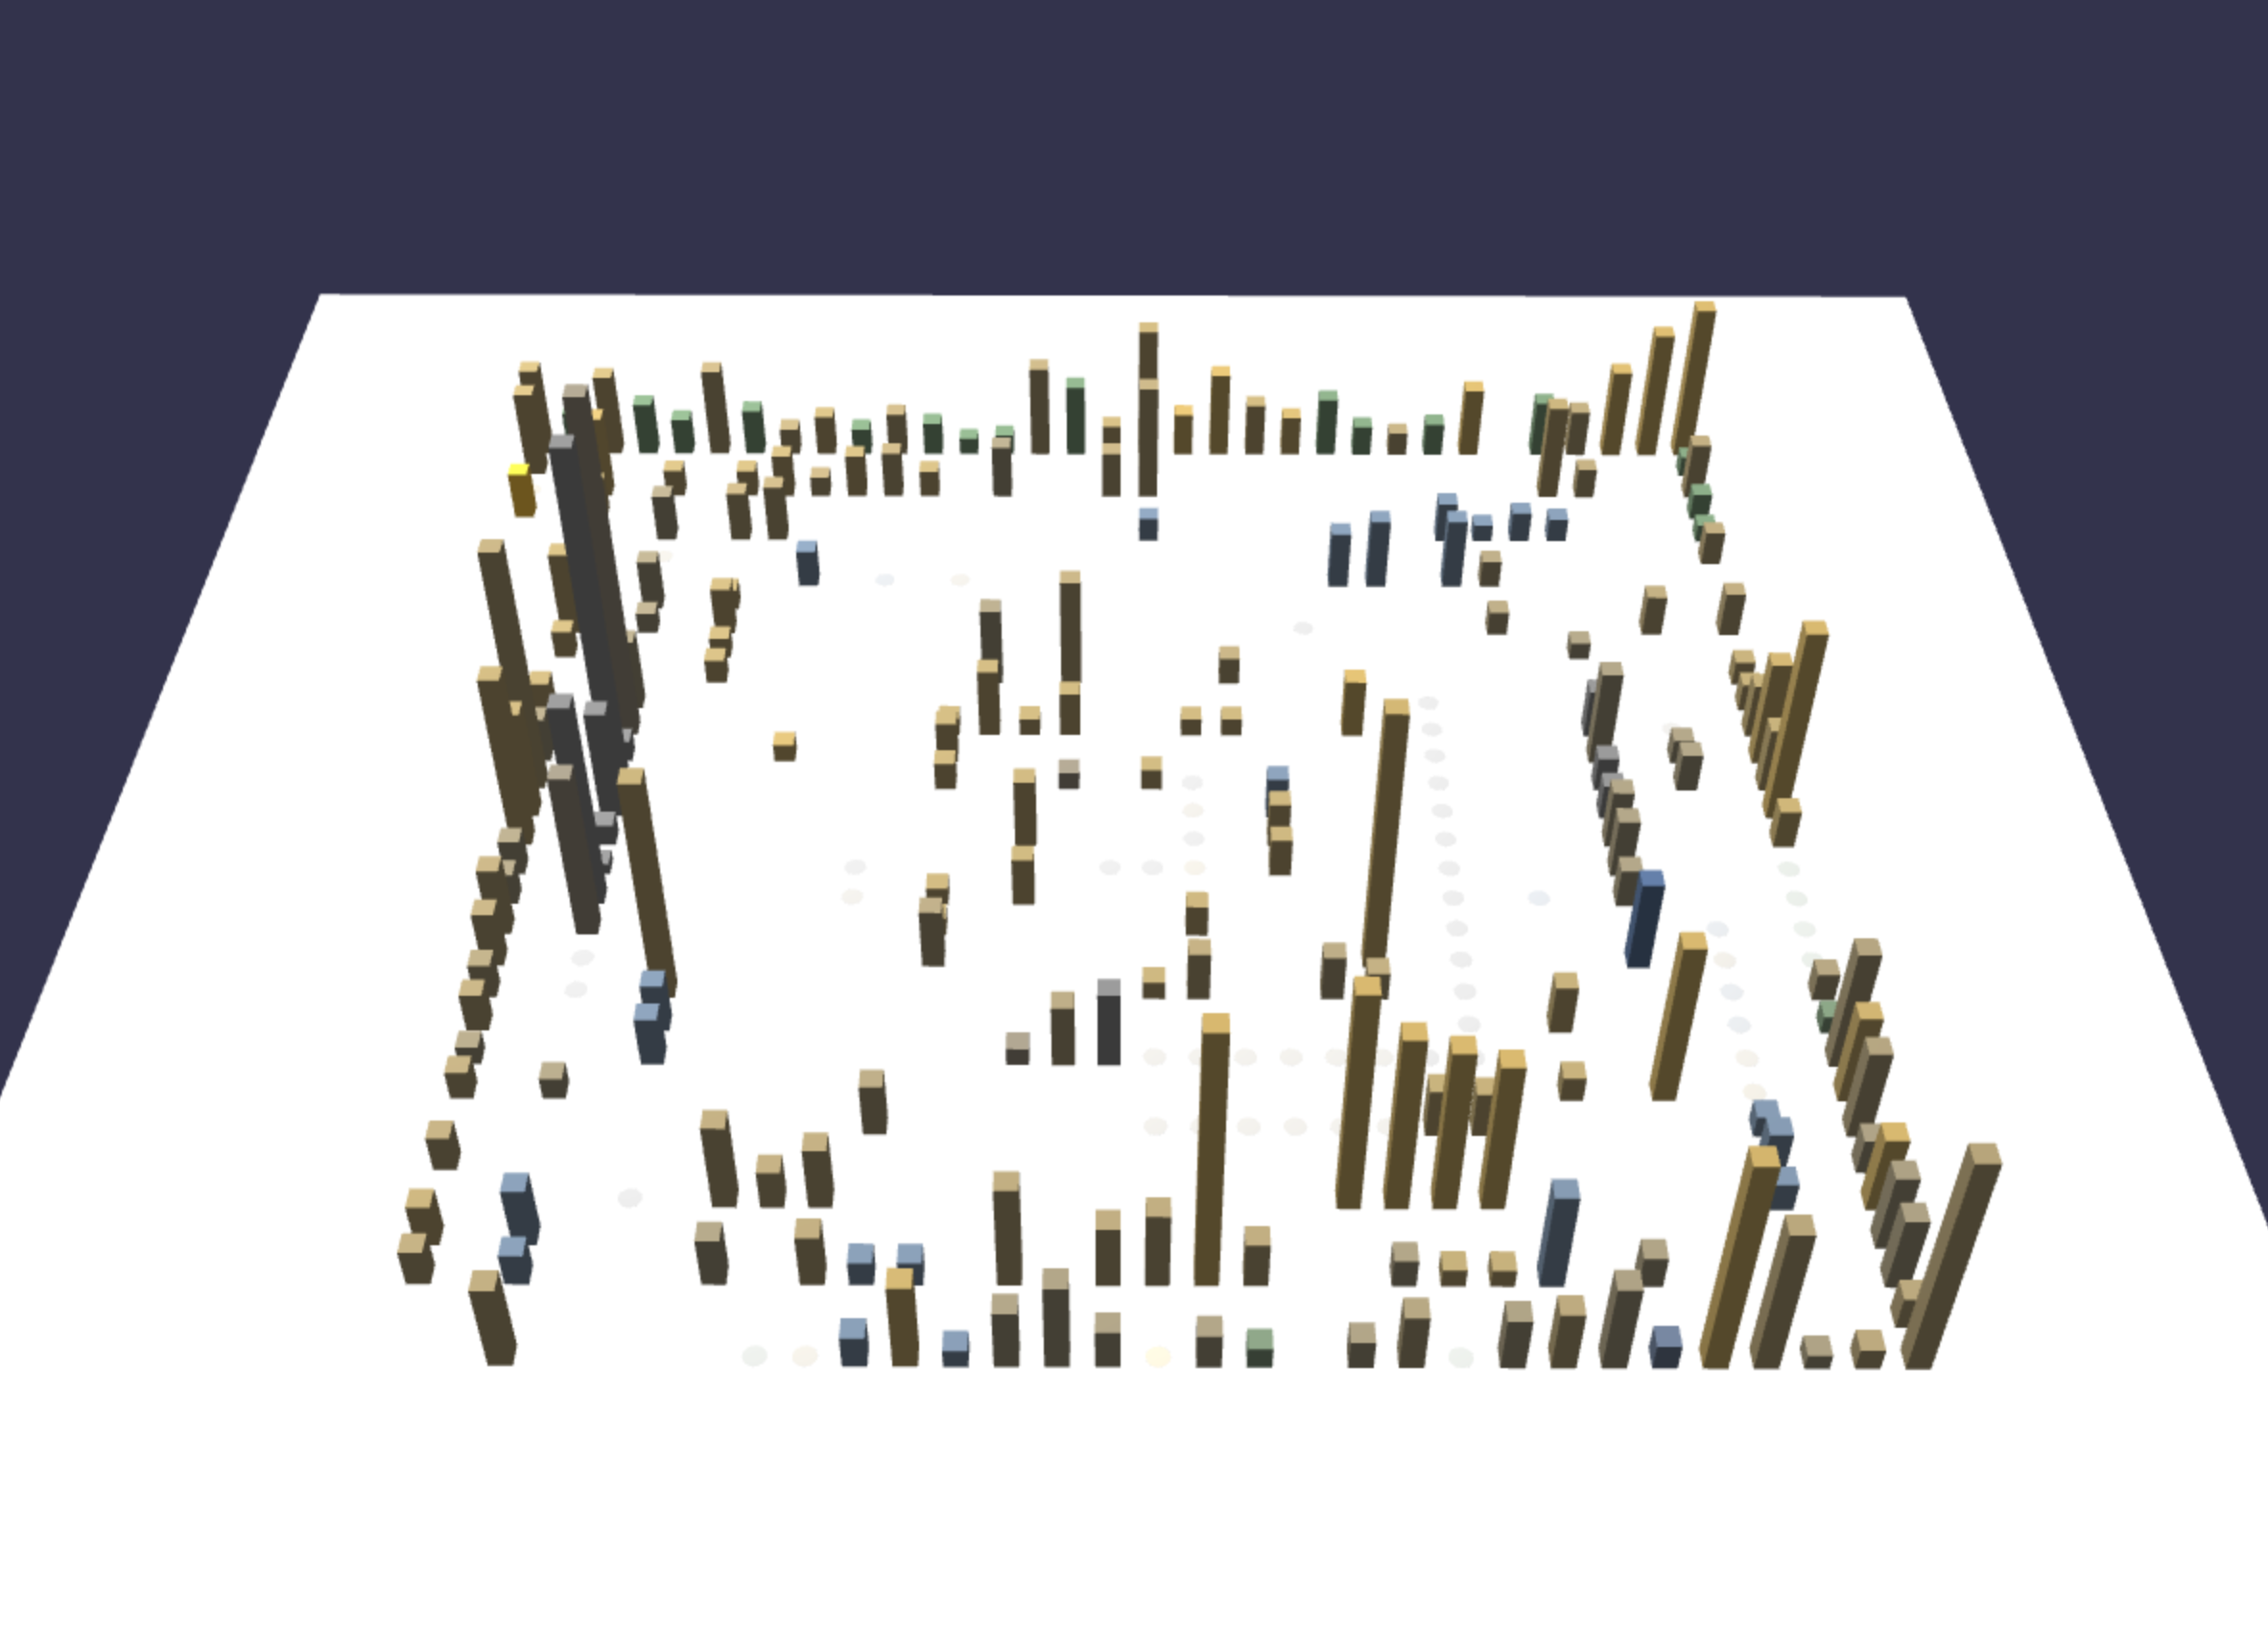
\includegraphics[width=\linewidth]{JetUML_V3S4.png}
        \caption{Year 4} 
        \label{fig:JetUML_V3S4}
    \end{subfigure}
        
    \caption{Evolution of JetUML} 
    \label{fig:JetUML_V3}
\end{figure}

\begin{figure}[h!]    \ContinuedFloat
    \begin{subfigure}{0.48\textwidth}
        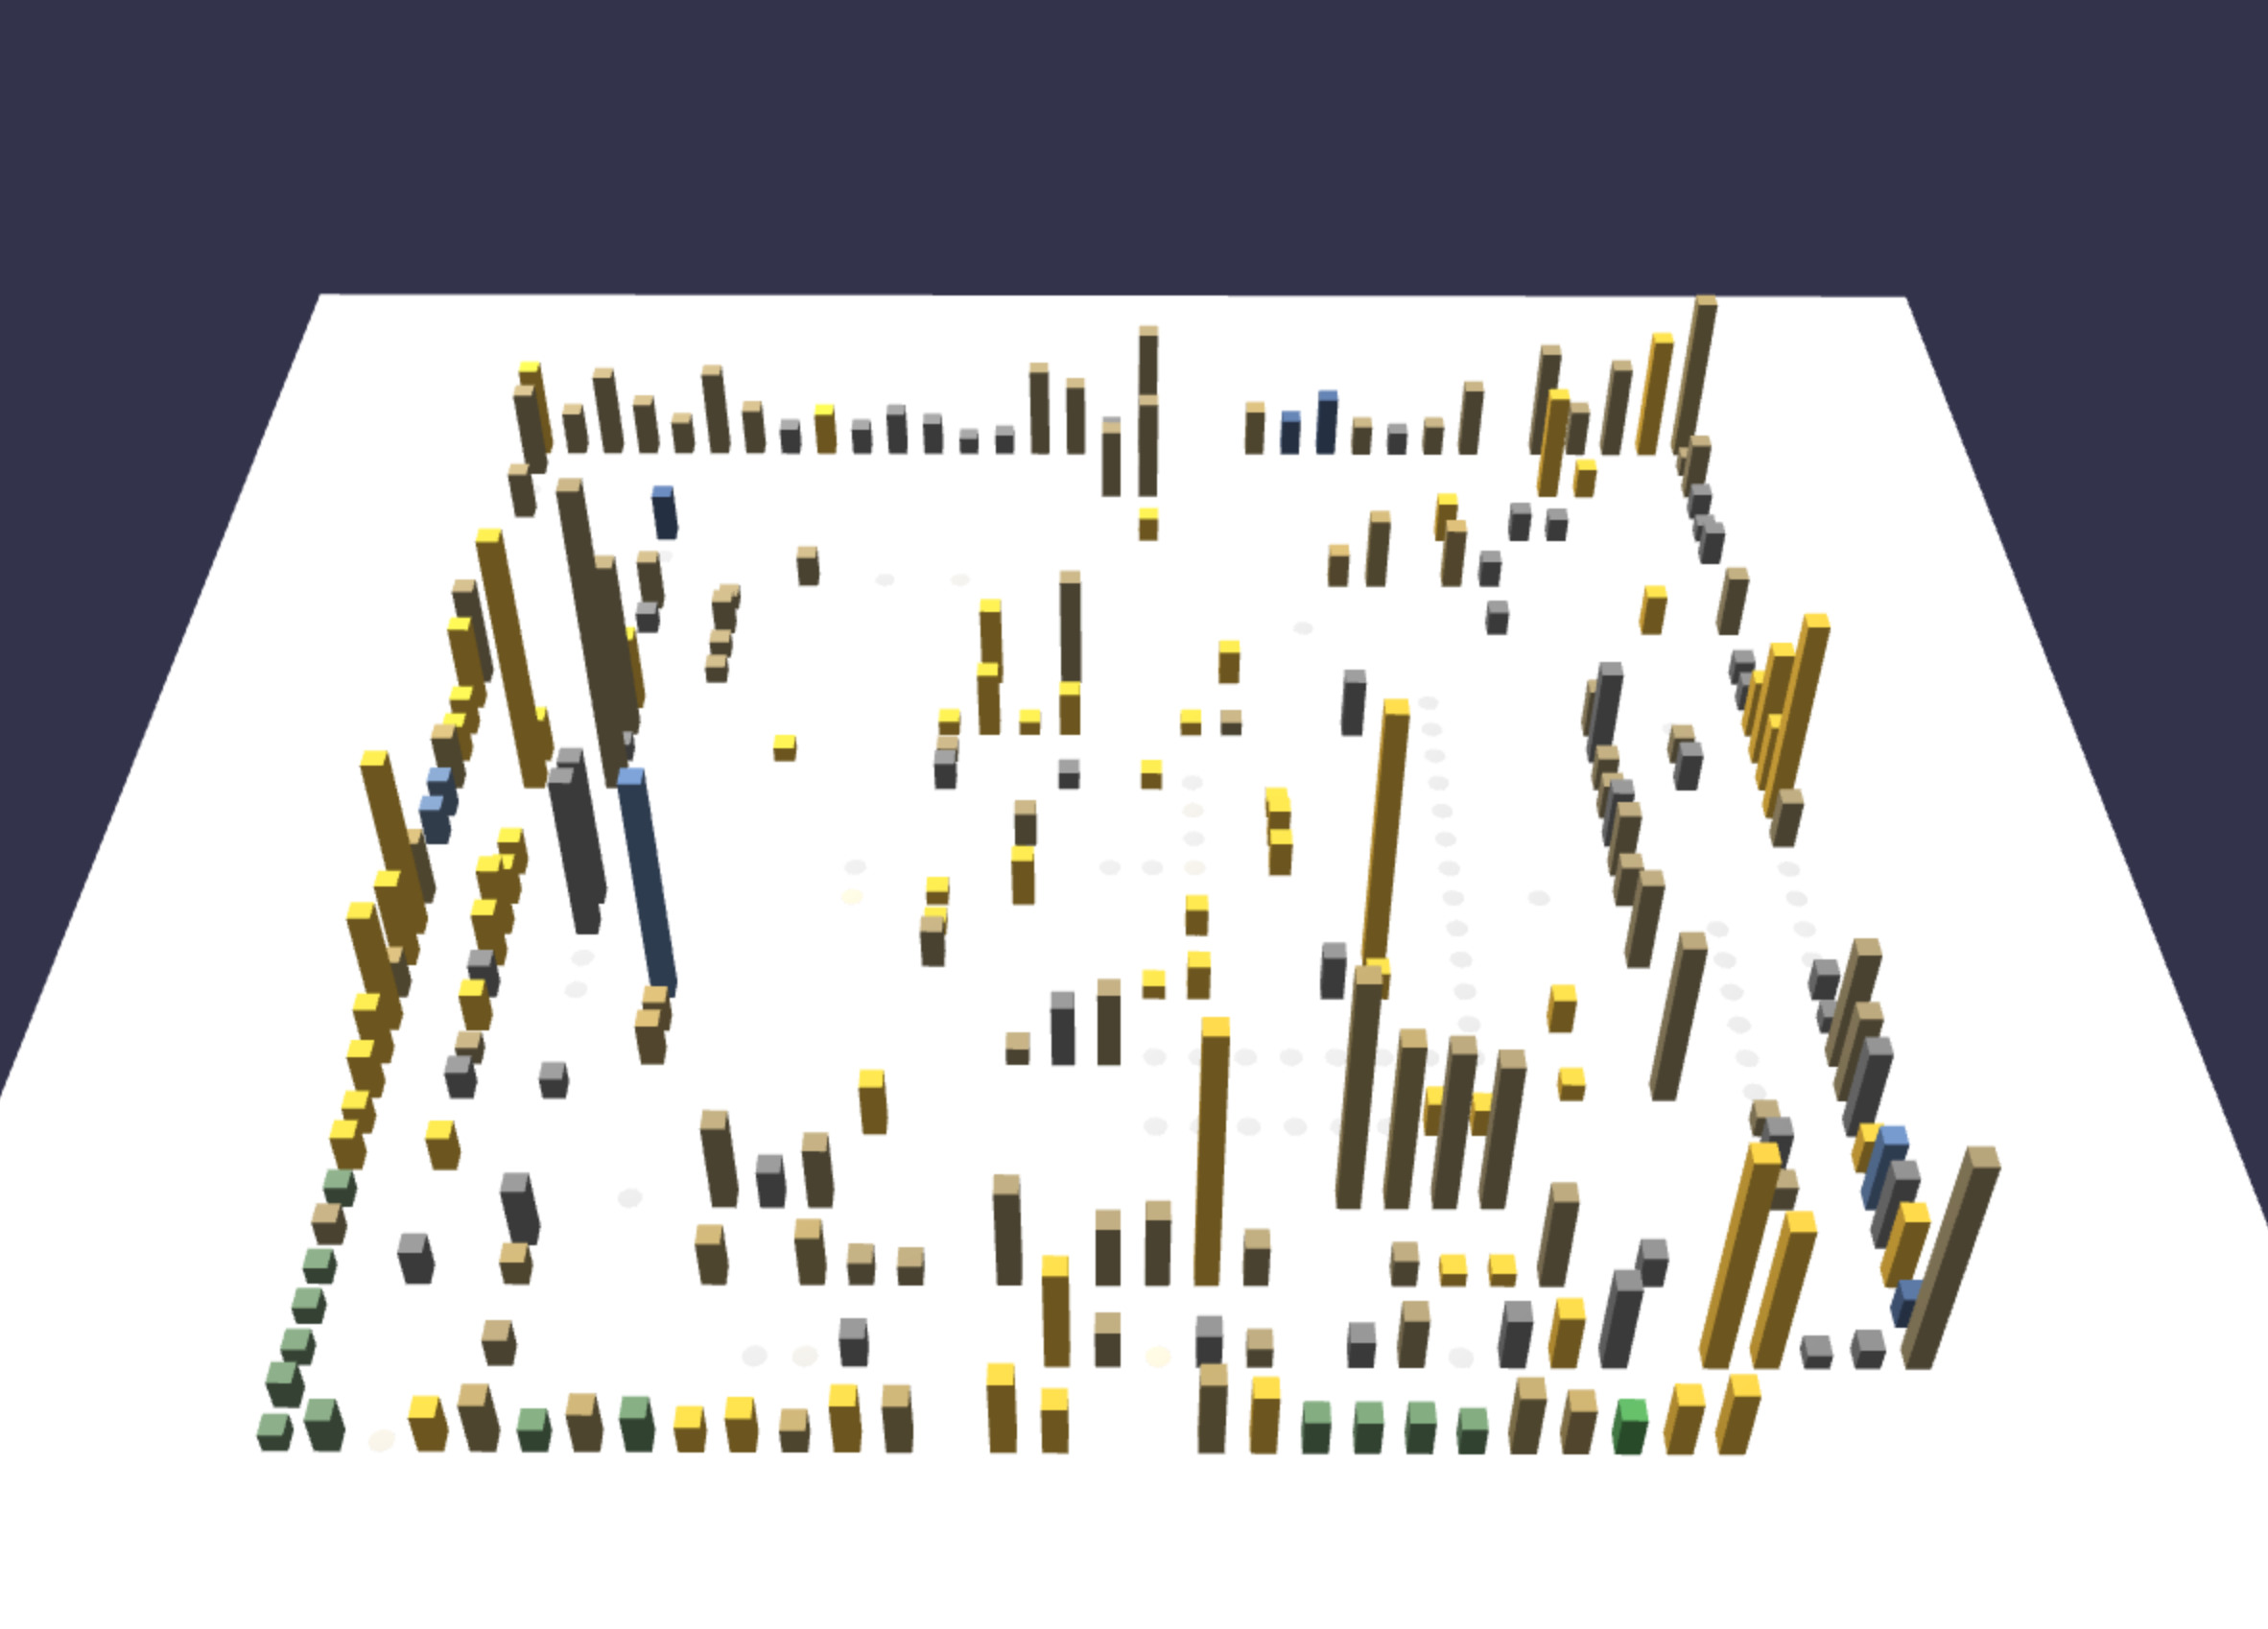
\includegraphics[width=\linewidth]{JetUML_V3S5.png}
        \caption{Year 5} 
        \label{fig:JetUML_V3S5}
    \end{subfigure}\hspace*{\fill}
    \begin{subfigure}{0.48\textwidth}
        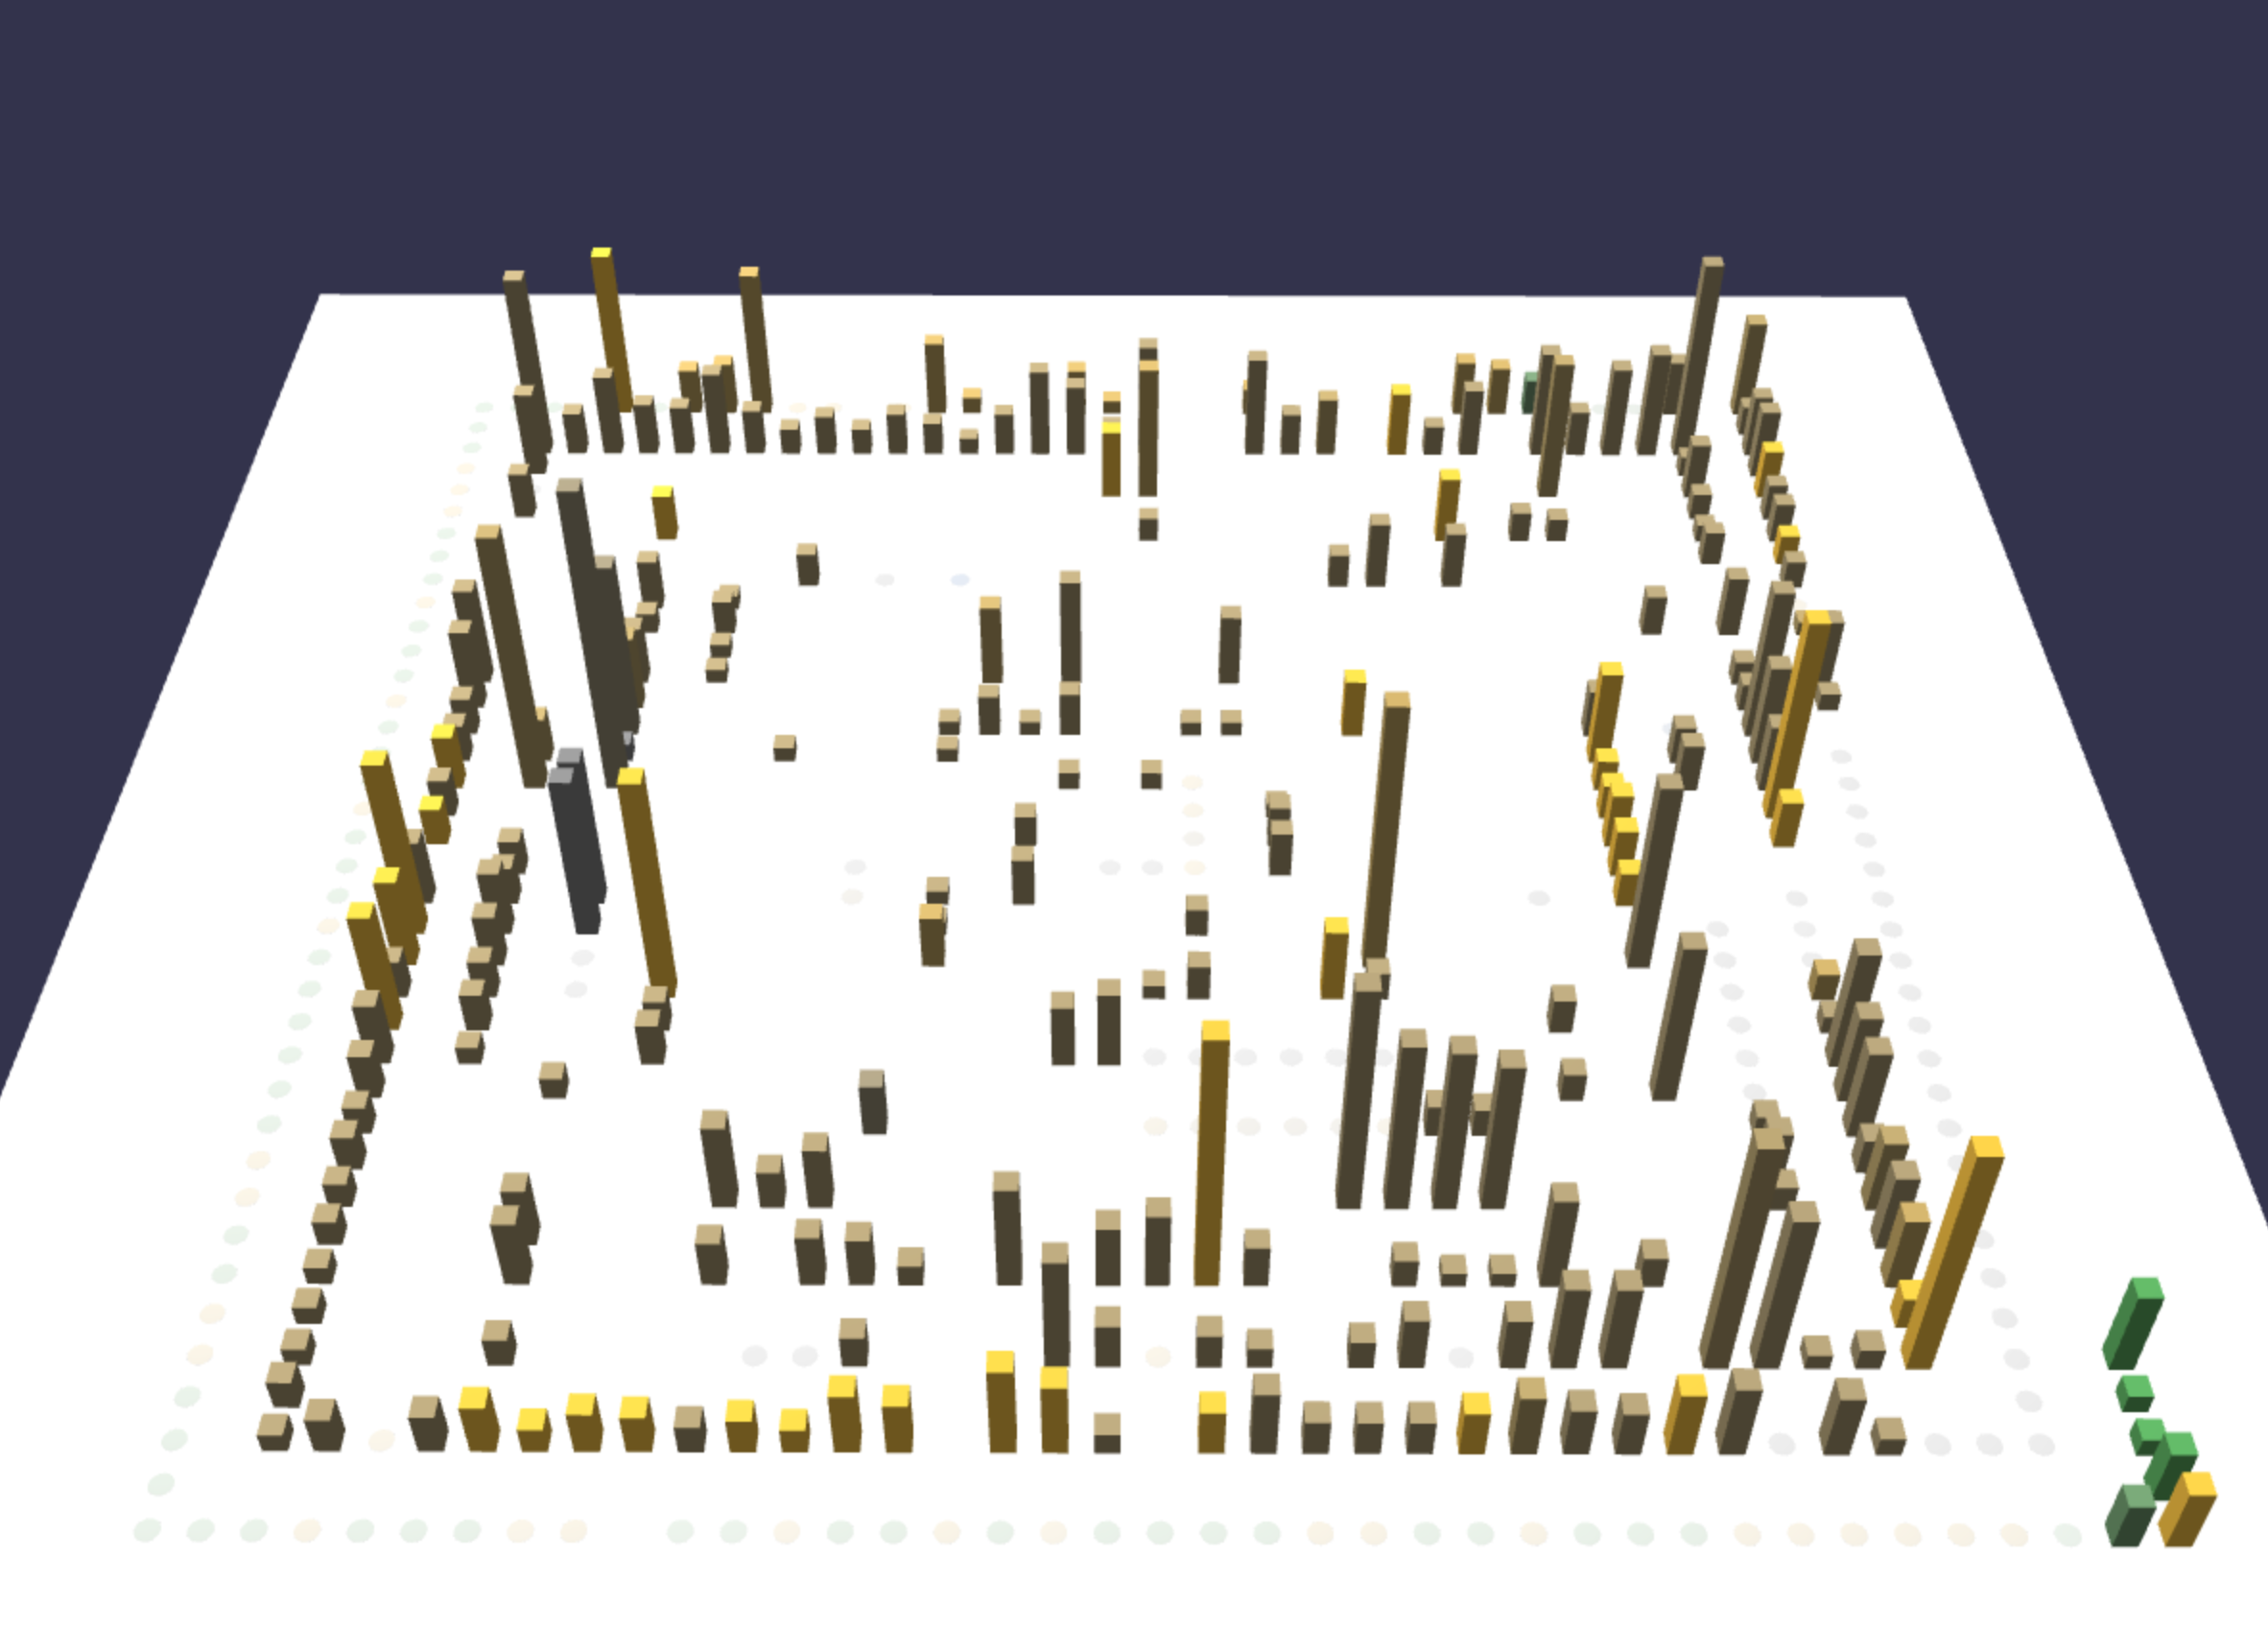
\includegraphics[width=\linewidth]{JetUML_V3S6.png}
        \caption{Year 6} 
        \label{fig:JetUML_V3S6}
    \end{subfigure}

    \medskip
    \begin{subfigure}{0.48\textwidth}
        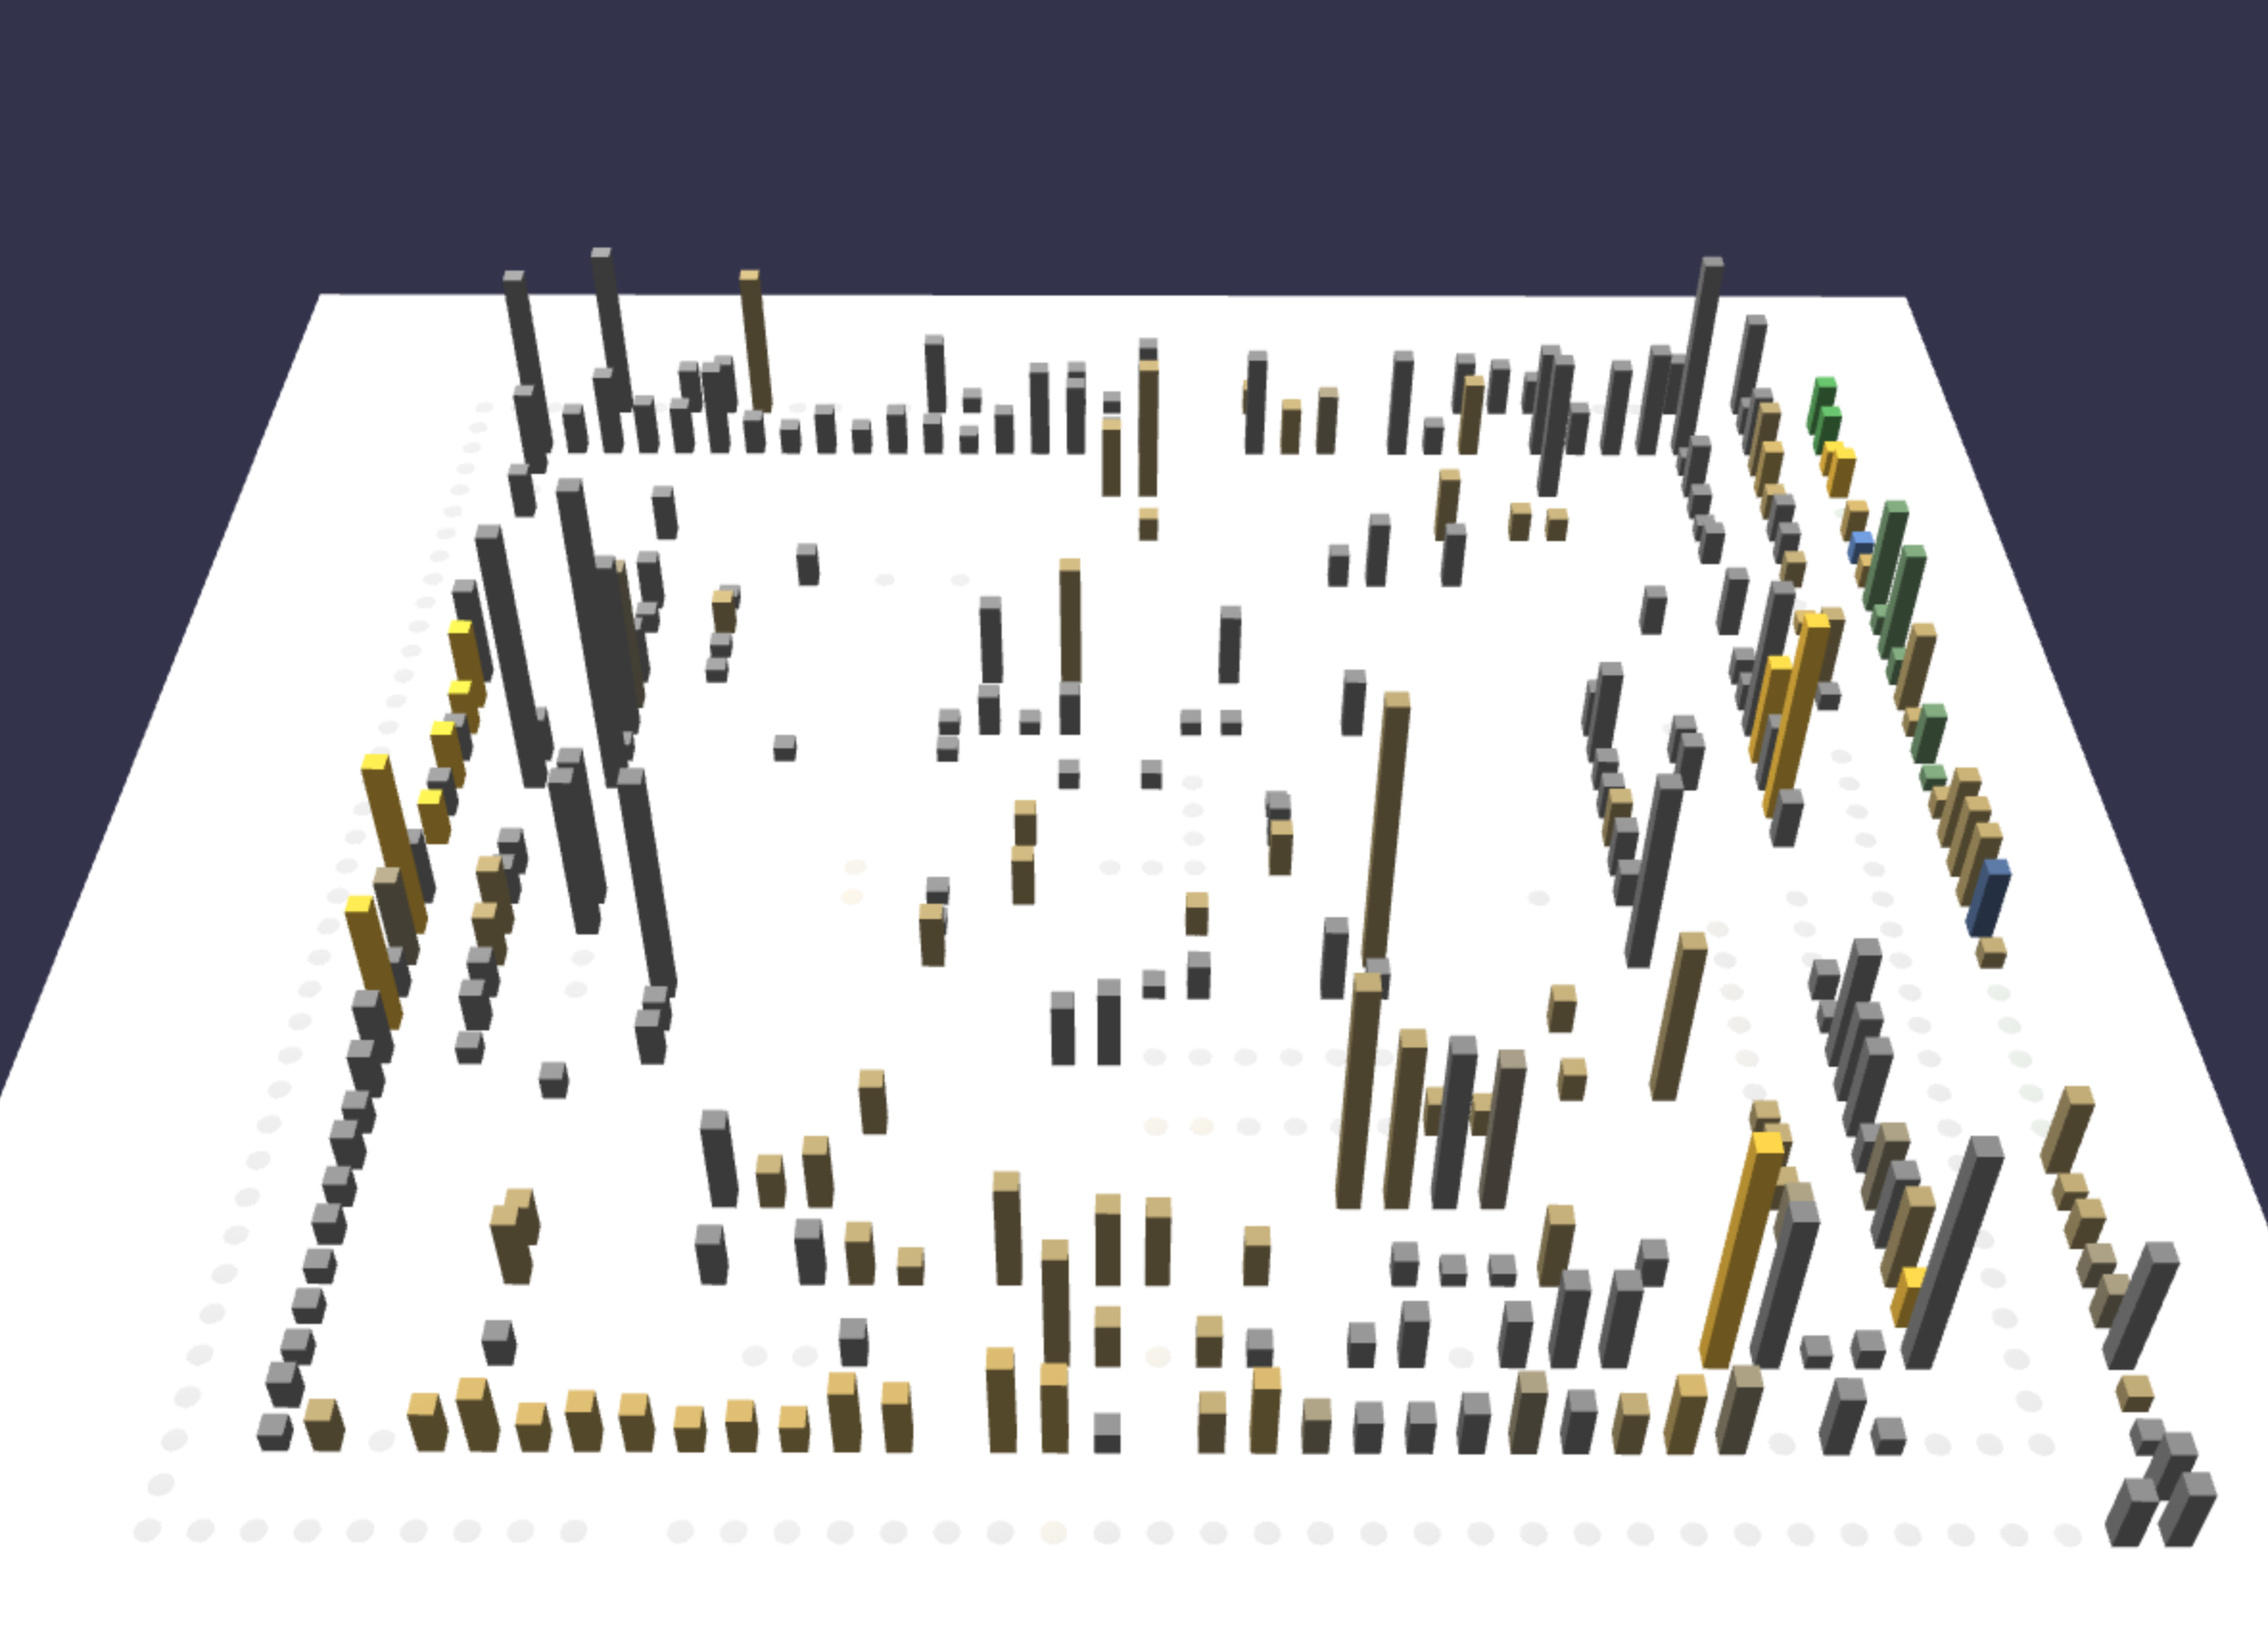
\includegraphics[width=\linewidth]{JetUML_V3S7.png}
        \caption{Year 7} 
        \label{fig:JetUML_V3S7}
    \end{subfigure}\hspace*{\fill}
    \begin{subfigure}{0.48\textwidth}
        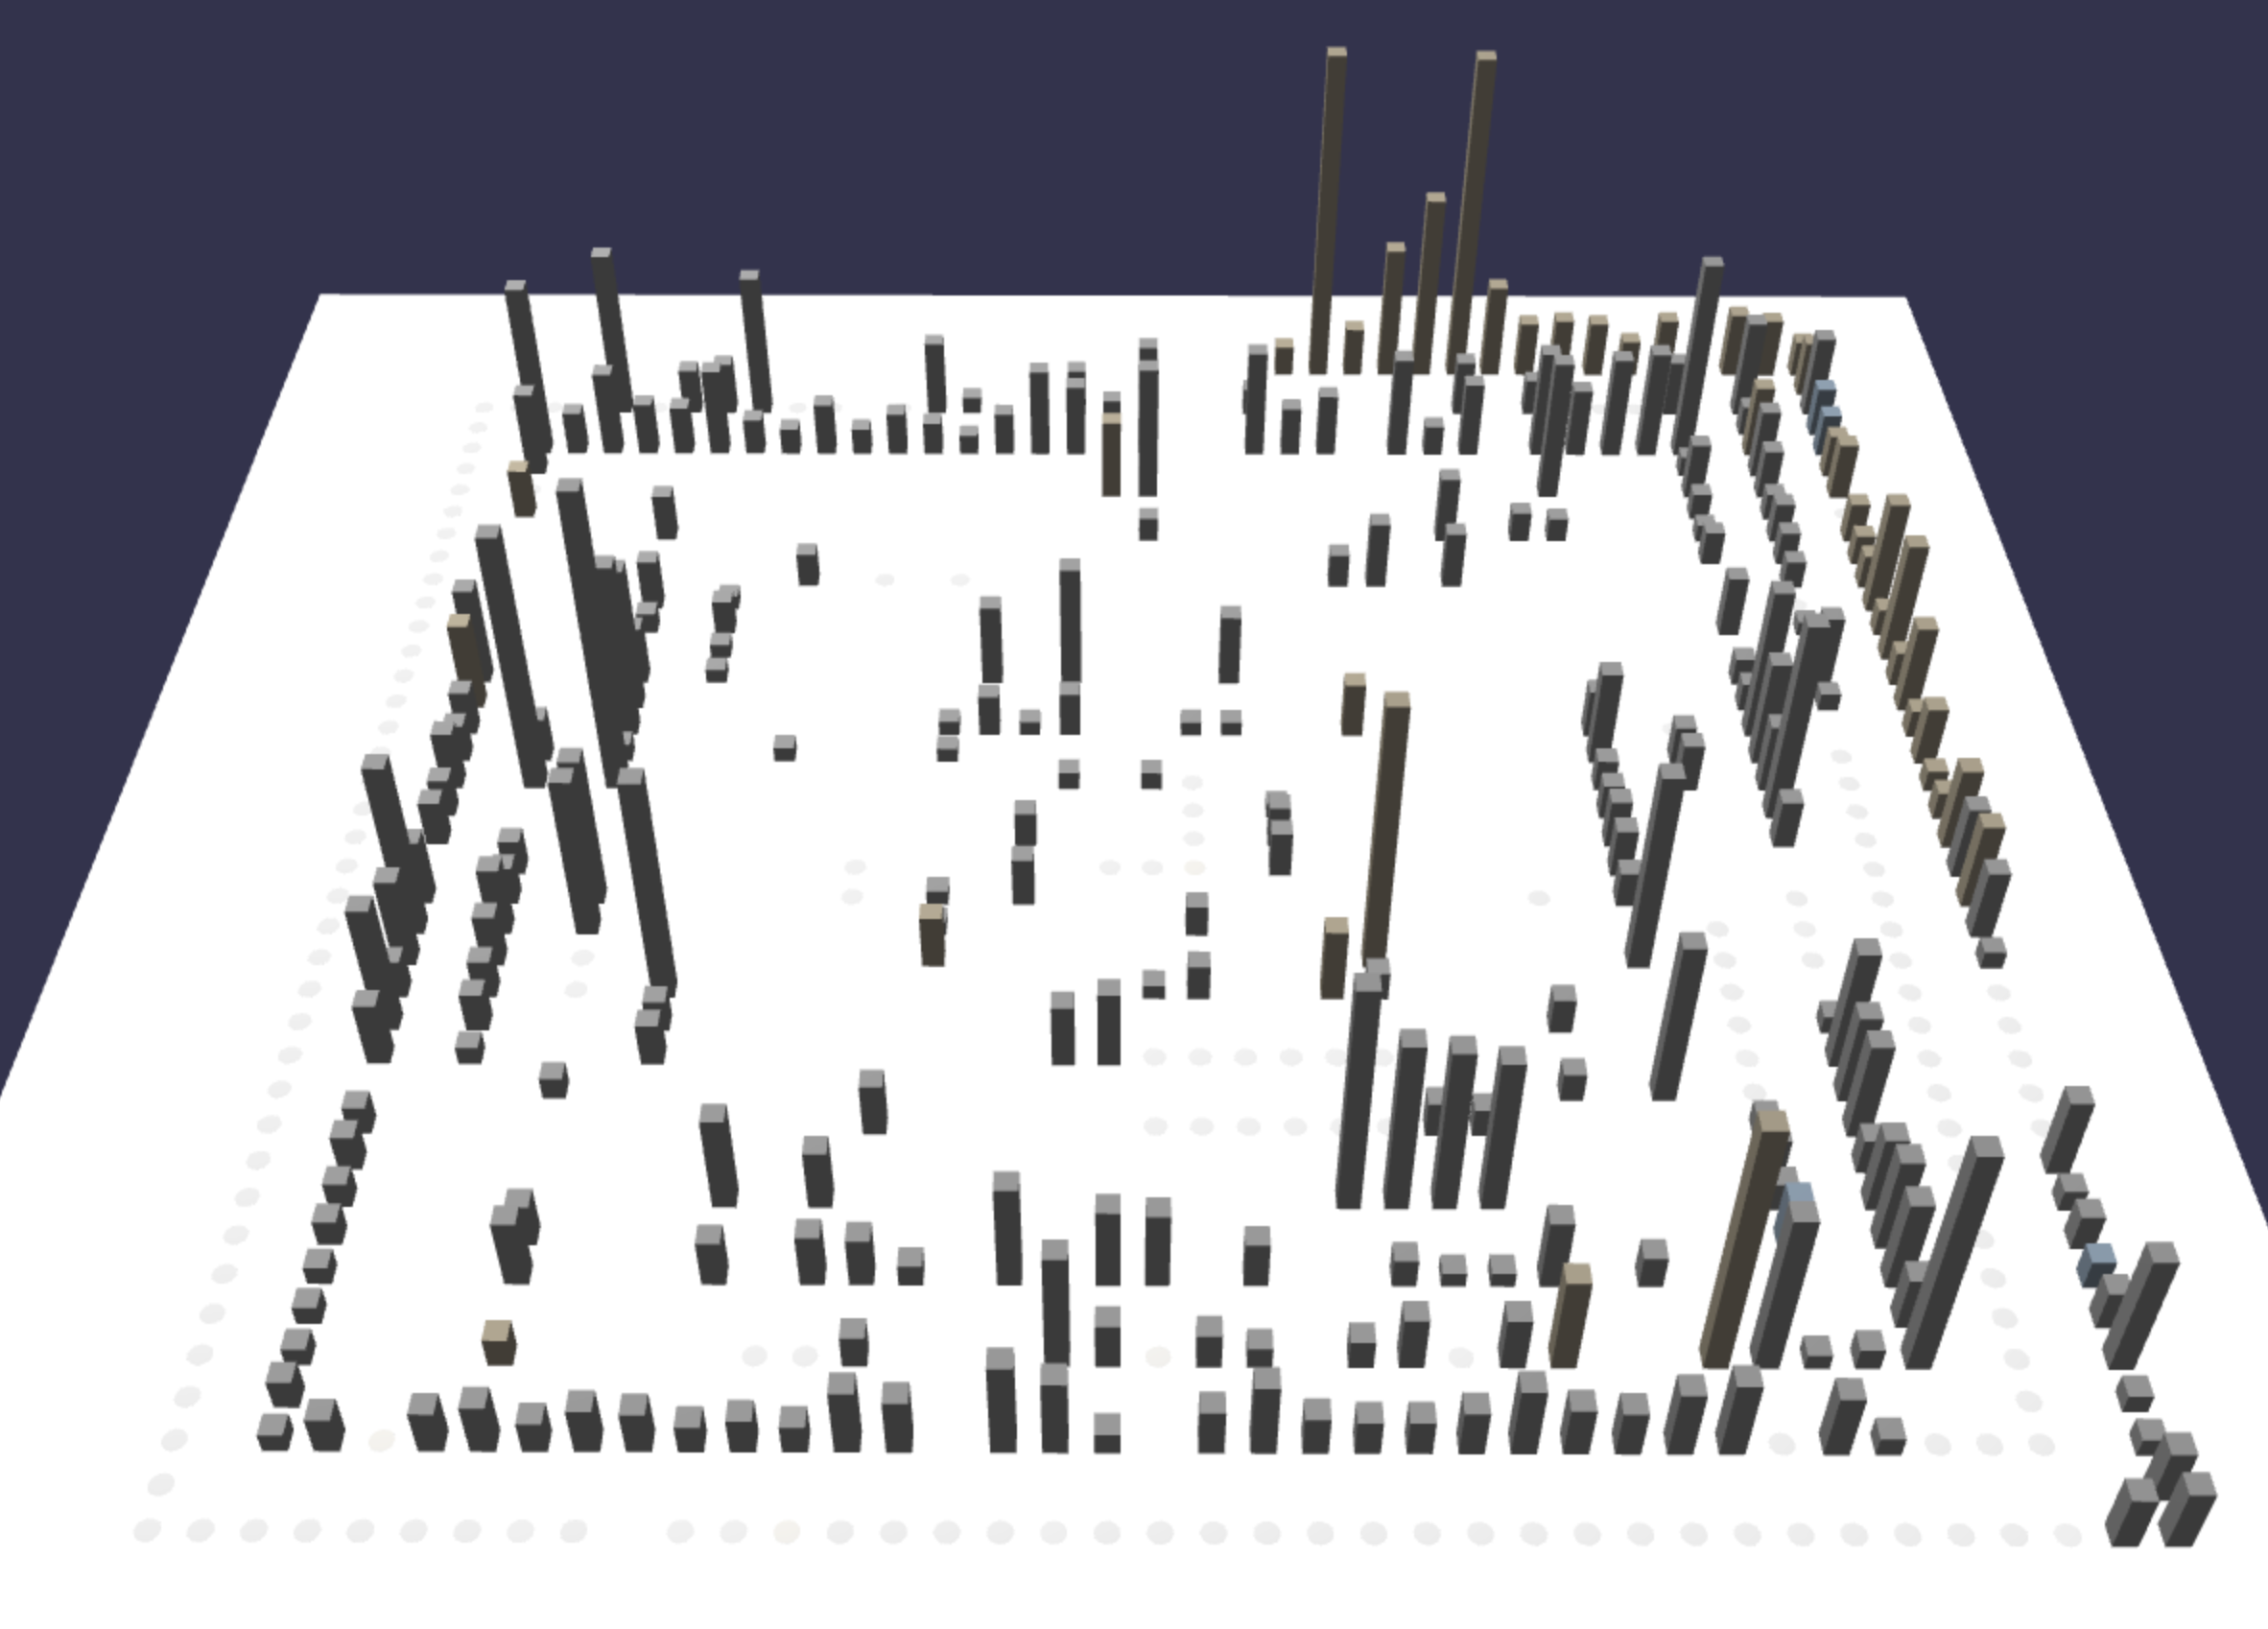
\includegraphics[width=\linewidth]{JetUML_V3S8.png}
        \caption{Year 8 (last)} 
        \label{fig:JetUML_V3S8}
    \end{subfigure}
    
    \caption{Evolution of JetUML} 
    \label{fig:JetUML_V3}
\end{figure}
